\documentclass[letterpaper, 10 pt, twocolumn, conference]{article}

\usepackage[paper=letterpaper,left=19.1mm,right=19.1mm,width=7in,top=19.1mm,bottom=19.1mm]{geometry}
%\usepackage{mathptmx} % assumes new font selection scheme installed
\usepackage{newtxmath}
\usepackage{times} % assumes new font selection scheme installed

\usepackage{multirow}
\usepackage{setspace} % This is used in the title page
\usepackage{array}
\usepackage{caption}
\usepackage{subcaption}
\usepackage{listings}
\usepackage{amsmath, amssymb, graphics, setspace}
\usepackage{caption}
%\usepackage{algorithmic}
\usepackage[ruled,vlined]{algorithm2e}
\usepackage[noend]{algpseudocode}
\usepackage{longtable}
\usepackage{natbib}
\bibliographystyle{plainnat}
%\usepackage{section}{placeins}
\usepackage{float}
\usepackage{hyperref}
\usepackage[section]{placeins}
\usepackage[pdftex]{graphicx}
\usepackage{epstopdf}
%\usepackage{epsfig}

%% END OF USER ADDED PACKAGES

%% User command 
\makeatletter
\newcommand{\algorithmicinput}{\textbf{Parameters:}}
\newcommand{\Input}{\item[\algorithmicinput]}
\makeatother

\let\oldhat\hat
\renewcommand{\vec}[1]{\boldsymbol{#1}}
\renewcommand{\hat}[1]{\oldhat{\mathbf{#1}}}

%to make vertical spacing of algorithm environment larger or smaller
\algrenewcommand\alglinenumber[1]{{\sffamily\footnotesize#1}}
\makeatletter
%\xpatchcmd{\algorithmic}{\itemsep\z@}{\itemsep=0.7ex}{}{} %..ex value decides about the algorithm environment spacing
\makeatother

\renewcommand{\algorithmiccomment}[1]{\bgroup\hfill\scriptsize//~#1\egroup}

\makeatletter
\let\OldStatex\Statex
\renewcommand{\Statex}[1][3]{%
  \setlength\@tempdima{\algorithmicindent}%
  \OldStatex\hskip\dimexpr#1\@tempdima\relax}
\makeatother

\restylefloat{figure}

%% END user commands

\title{\LARGE \bf
A Recipe for Soft Fluidic Elastomer Robots
}

\author{Andrew D. Marchese, Robert K. Katzschmann, and Daniela Rus% <-this % stops a space
\thanks{Andrew D. Marchese, Robert K. Katzschmann, and Daniela Rus are with the Computer Science and Artificial Intelligence Laboratory, Massachusetts Institute of Technology, 32 Vassar St, Cambridge, MA 02139, USA, {\tt\small \{andy, rkk, rus\}@csail.mit.edu}}%
}

\begin{document}

\maketitle
\thanks
%\twocolumn[
  %\begin{@twocolumnfalse}
    \begin{abstract}
	\textbf{
      	This work provides approaches to designing and fabricating soft fluidic elastomer robots.
%
%That is, novel approaches to design, fabrication, kinematic modeling, power, control, and planning as well as extensive experimental evaluations with multiple manipulator prototypes are presented.
%
That is, three viable actuator morphologies composed entirely from soft silicone rubber are explored, and these morphologies are differentiated by their internal channel structure, namely: ribbed, cylindrical, and pleated.
%
Additionally, three distinct casting-based fabrication processes are explored: lamination-based casting, retractable-pin-based casting, and lost-wax-based casting.
%
Furthermore, two ways of fabricating a multiple DOF manipulator are explored: casting the complete manipulator as a whole, and casting single DOF segments with subsequent concatenation.
%
We experimentally validate each soft actuator morphology and fabrication process by creating multiple physical soft manipulator prototypes.

%An approach to closed-loop configuration control is presented using a piecewise constant curvature kinematic model, real-time localization data, and novel fluidic drive cylinders which power actuation.
%%
%Multi-segment forward and inverse kinematic algorithms are developed and combined with the configuration controller to provide reliable task-space position control.
%%
%Building on these developments, a suite of task-space planners are presented to demonstrate new autonomous capabilities from these soft robots such as: (i) tracking a path in free-space, (ii) maneuvering in confined environments, and (iii) grasping and placing objects.
%%
%Extensive evaluations of these capabilities with physical prototypes demonstrate for the first time that manipulation with soft fluidic elastomer robots is viable.

	}
    \end{abstract}
    %\bigskip
  %\end{@twocolumnfalse}
%]
%\thispagestyle{empty}
%\pagestyle{plain}


\section{Introduction}
\label{sec:Introduction}
%%%%%%%%%%%%%%%%%%%%% Vision %%%%%%%%%%%%%%%%%%%%%%%%%
The goal of this work is to provide and compare multiple actuator morphologies and multiple fabrication processes for realizing soft autonomous fluidic elastomer robots.
%
We experimentally validate these morphologies and processes in the context of extremely soft and highly compliant locomotory robots and manipulators shown in Figure~\ref{fig:intro_new}.
\begin{figure}[!t]
  \centering
  \includegraphics[width=3in]{figures/introduction/intro_new.eps}
  \caption{Extremely soft and highly compliant fluidic elastomer robots. (\textbf{a}) Ribbed planar manipulator \citep{marchese2014design}, (\textbf{b}) Cylindrical planar manipulator \citep{marchese2014whole}, (\textbf{c}) Cylindrical manipulator with gripper \citep{katzschmann2015autonomous}, (\textbf{d}) Self-contained pneumatic fish \citep{marchese2014autonomous}(photo courtesy of Devon Jarvis for popular mechanics), (\textbf{e}) Spatial cylindrical manipulator \citep{marchese2015design}, and (\textbf{f}) Self-contained hydraulic fish \citep{katzschmann2014hydraulic}. }\label{fig:intro_new}
\end{figure}

Soft robots exhibit continuum body motion, large scale deformation, and relatively high compliance compared to traditional rigid-bodied robots \citep{trivedi2008soft}.
%
Such characteristics give this class of robots advantages like the ability to mitigate uncertainty with passive compliance \citep{mcmahan2006field}, perform highly dexterous tasks \citep{deimel2014novel}, and exhibit resiliency \citep{tolley2014resilient}.
%
This work provides a recipe for designing and fabricating soft fluidic elastomer actuators and robotic systems.

%%%%%%%%%%%%%%%%%%%%% Challenges %%%%%%%%%%%%%%%%%%%%%%%%%
\subsection{Challenges}
Recent reviews \citep{trivedi2008soft, trimmer2014journal, lipson2014challenges, majidi2014soft} articulate the challenges associated with creating robots from soft, nonlinear materials.
%
To summarize, current engineering tools are well-suited for rigid-bodied robots and when soft, nonlinear elastic materials are introduced, many of the underlying assumptions of these tools are broken.
%
To create fluidic elastomer robots, we must overcome many technical challenges, many of which have to do with design and fabrication.
%
More specifically, this work addresses the following challenges:
(i) We do not have multi-segment fluidic elastomer locomotory robot nor manipulator designs suitable for automated tasks.
That is, we need to identify appropriate actuator morphologies and ways of assembling these actuators into multi-body robots.
(ii) Consistently reproducing certain properties of soft robots, for example their elasticity or internal channel geometry, is difficult using conventional fabrication techniques.
Accordingly, we must develop fabrication techniques that balance the competing goals of scalability and repeatability with the need for complicated features and shape profiles.

%%%%%%%%%%%%%%%%%%%%% Approach %%%%%%%%%%%%%%%%%%%%%%%%%
\subsection{Approach}
%In this work, we demonstrate that autonomous manipulation with soft fluidic elastomer robots is possible.
First, we review relevant soft actuation technology, design tools, and fabrication processes in Section~\ref{sec:Related Work}.
%
Next, we present the design and characterization of three fluidic elastomer actuator morphologies in Section~\ref{sec:Actuators}.
%
These actuator morphologies are differentiated by their internal channel structure, namely: ribbed, cylindrical, and pleated.
%
Next, we provide three alternative fabrication approaches for reliably fabricating soft actuators and multi-segment robots in Section~\ref{sec:Fabrication}.
%
These processes are lamination-based embedded casting, retractable-pin-based casting, and lost-wax-based casting.
%
Then, we briefly discuss alternative approaches to powering these robots in Section~\ref{sec:Power}.
%
And lastly, we demonstrate how the various actuator morphologies and fabrication processes have been used to realize a variety of soft autonomous systems: locomotory fish-like robots in Section~\ref{sec:Locomotion} and robotic manipulation systems in Section~\ref{sec:Manipulators}.

%%%%%%%%%%%%%%%%%%%%% Contributions %%%%%%%%%%%%%%%%%%%%%%%%%
\subsection{Contributions}
%The primary contribution of this work is a novel power and computational control and planning system for 2D fluidic elastomer manipulation that enable grasp-and-place and planned continuous motion in environments with obstacles.
%This work is first to show that planar manipulation with soft fluidic elastomer robots is possible and first to provide an approach for closed-loop control and planning of such manipulators.
Specifically this work makes the following contributions:
\begin{enumerate}
  \item Three viable fluidic elastomer actuator (FEA) morphologies. That is, a FEA with a (i) ribbed channel structure and embedded transmission lines, (ii) cylindrical channel structure and hollow interior, (iii) seamless pleated channel structure;
  \item Three fabrication processes for reliably manufacturing these FEAs. These are (i) a lamination-based casting process with heterogeneous embedded components, (ii) a retractable-pin-based casting process, (iii) a lost-wax-based casting process;
  \item A survey of recent robots built using these design and fabrication approaches (See Fig.~\ref{fig:intro_new}).
\end{enumerate}
This work significantly extends three previous conference publications: \citep{marchese2014design}, \citep{marchese2014whole}, and \citep{katzschmann2015autonomous} (in revision). %TODO remove if not in revision anymore 

\section{Related Work}
\label{sec:Related Work}

This paper builds on several recent results in the design and fabrication of soft robots; see \citep{lipson2013challenges}, \citep{rus2014soft}, \citep{marchese2015thesis} for detailed reviews.

\subsection{Actuation}
\label{subsec:RW Actuation}
There are various approaches to actuating the body of a soft robot.
One distinguishing feature of many soft robots is that actuators and/or power transmission systems are integrated within and distributed throughout the body.
In the following we review four common actuator types, and these are also depicted in Figure~\ref{fig:RW actuation}.
\begin{figure}
  \centering
  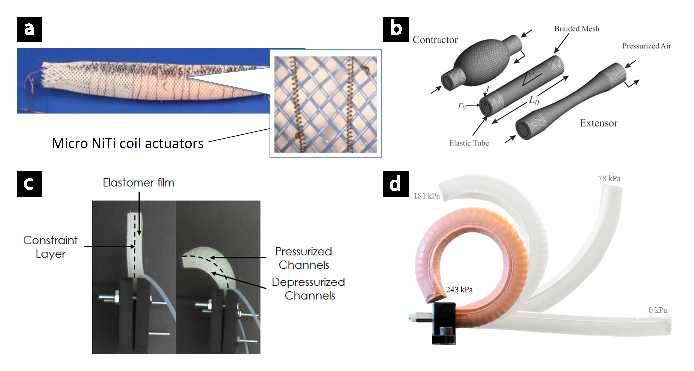
\includegraphics[width=3in]{figures/relatedwork/actuation.eps}
  \caption[Common actuation approaches for soft robots.]{Common actuation approaches for soft robots. (\textbf{a}) Shape Memory Alloy (SMA) actuators \citep{seok2010peristaltic}, (\textbf{b}) Pneumatic Artificial Muscle (PAM) actuators \citep{mcmahan2006field}, (\textbf{c}) Fluidic Elastomer Actuators (FEAs) \citep{onal2011soft}, and (\textbf{d}) Fiber reinforced FEAs \citep{galloway2013mechanically}.}\label{fig:RW actuation}
\end{figure}

\subsubsection{Shape Memory Alloy Actuators}
\label{subsubsec:RW SMA}
\hl{The basic operating principle behind Shape Memory Alloy (SMA) technology is that nickel titanium (NiTi) wire contracts under joule heating.
This heating is typically produced by passing electrical current through the wire.
The contracting wire can be used as an agonist actuator, similar to the way one's bicep pulls the forearm towards the body.
\mbox{\citet{kim2009micro}} model, design, and fabricate these actuators and show their viability in soft robot applications.
Additionally, the elastomer-based bio-inspired octopus arms developed in \mbox{\citet{laschi2012soft}} and \mbox{\citet{cianchetti2014bioinspired}} use SMA actuation to emulate a muscular hydrostat.
Further, \mbox{\citet{seok2010peristaltic}} use SMA spring actuators to generate peristaltic locomotion in a worm-like robot (see Fig.~\mbox{\ref{fig:RW actuation}}a), \mbox{\citet{koh2013omega}} develop SMA coil-spring actuators to generate two-anchor crawling in an inchworm-like robot, and \mbox{\citet{umedachi2013highly}} use SMA actuators to produce both crawling and inching in 3D printed soft robot.}


\subsubsection{Cable Actuators}
\label{subsubsec:RW Cables}
Originally, many hard hyper redundant and hard continuum robots \citep{cieslak1999elephant, buckingham2002snake, gravagne2002uniform, hannan2003kinematics, mcmahan2005design, camarillo2009configuration} used an array of servomotors or linear actuators to pull cables that move rigid connecting plates located between body segments.
Some softer robots have adopted a similar actuation scheme consisting of tendons pulling rigid fixtures embedded within an elastomer body.
\hl{For example, the soft-bodied fish developed by \mbox{\citet{youcef2006design}}, the soft octopus-inspired arms developed in \mbox{\citet{calisti2010study}} and \mbox{\citet{calisti2011octopus}}, as well as the soft arm developed by \mbox{\citet{wang2013visual}} use this actuation approach.}

\subsubsection{Pneumatic Artificial Muscles}
\label{subsubsec:RW PMA}
Another common actuation scheme for soft robots involves distributed Pneumatic Artificial Muscle (PAM) actuators, also known as McKibben actuators and shown in Figure~\ref{fig:RW actuation}b.
A PAM is fundamentally composed of an inflatable elastic tube surrounded by a braided mesh.
Depending on the weave pattern of the braided mesh, the actuator can be designed to contract or extend under input pressure.
Typically, these actuators are operated with driving pressures between 50 to 100 ~psi.
\hl{These actuators have been used and studied extensively in \mbox{\citet{chou1996measurement, tondu2000modeling}} \mbox{\citet{caldwell2000bio, daerden2002pneumatic}} and \mbox{\citet{reynolds2003modeling}}.}
Notable semi-soft robots using PAMs include \citet{mcmahan2006field, pritts2004design} and \citet{kang2013design}.

\subsubsection{Fluidic Elastomer Actuators}
\label{subsubsec:RW FEA}
A softer alternative is the Fluidic Elastomer Actuator (FEA), which is used predominantly throughout this paper (see Fig.~\ref{fig:RW actuation}c).
The FEA is an actuator composed of low durometer rubber and driven by relatively low-pressure fluid in the range of 3 to 8~psi.
\hl{Although many motion primitives are achievable with a FEA (e.g., extending, contracting, twisting, and bending) in this work we primarily focus on actuators designed for bending.}
Its basic structure consists of two soft elastomer layers separated by a flexible, but relatively inextensible constraint.
\hl{The inextensible constraint is typically created using cloth, paper, plastics, and even stiffer rubbers.}
Each of these elastomer layers contains embedded fluidic channels.
By pressurizing the fluid entrapped in these channels, stress is induced within the elastic material producing localized strain. This strain in combination with the relative in-extensibility of the constraint produces body segment bending.
FEAs can be powered pneumatically or hydraulically.

\hl{As the review by \mbox{\citet{rus2014soft}} discusses,} perhaps the earliest application of pneumatically actuated elastomer bending segments to robotics was by \citet{suzumori1992applying}.
Here fiber-reinforced Flexible Microactuators (FMAs) were developed and shown to be viable in a manipulator and multi-fingered hand.
\hl{Recently, these concepts have been extended and developed into the FEA and used to build a variety of soft mechanisms \mbox{\citep{shepherd2011multigait, ilievski2011soft, morin2012camouflage}}
\mbox{\citep{martinez2013robotic}}
and soft robotic systems
\mbox{\citep{onal2011soft, marchese2011soft, onal2013autonomous}}
\mbox{\citep{marchese2014autonomous, marchese2014design, marchese2014whole}}
\mbox{\citep{katzschmann2014hydraulic, katzschmann2015autonomous}}
\mbox{\citep{tolley2014untethered, tolley2014resilient}} \mbox{\citep{marchese2015design}}
\mbox{\citep{marchese2015control, marchese2015dynamics}}.}
Furthermore, \citet{polygerinos2013towards} and \citet{mosadegh2014pneumatic} have investigated more elaborate channel designs in order to reduce elastomer strain on the outer layer of the actuator, allowing for higher bending curvatures.
\hl{Additionally, \mbox{\citet{cianchetti2014soft}} develop a fluid actuated bending arm with a jamming \mbox{\citep{brown2010universal, liu1998nonlinear}} spine.}

There are also less flexible, fiber-reinforced FEAs (see Fig.~\ref{fig:RW actuation}d) that occupy the soft actuator space between purely elastomer FEAs and PAMs.
While these actuators have to operate with comparably higher driving pressures between 25 and 35~psi, they can accordingly apply higher forces which is advantageous for certain applications.
There are several notable examples of fiber-reinforced FEAs in the literature \citet{suzumori1992applying, suzumori2007bending, bishop2012design, galloway2013mechanically, deimel2013compliant, deimel2014novel} and \citet{park2014design}.

\subsection{Design Tools}
\label{subsec:RW Design Tools}
Design tools for soft robots are limited with respect to the availability of design tools for more traditional rigid-body robots.
\citet{suzumori2007bending} use Finite Element Modeling (FEM) to analyze the bending of fiber re-inforced pneumatic tube-like actuators.
Specifically, hyper-elastic material models are used to capture the nonlinear material properties of rubber, line elements are used to represent radial in-extensibility constraints due to fiber reinforcement, and the simulation is performed using the software MARC.
Outside of this example, the community has generally found that iterative nonlinear finite element solvers are limited to small deformations and of limited use when modeling very soft nonlinear materials \citep{lipson2014challenges}.
VoxCAD and the Voxelyze physics engine, as used in \citet{cheney2013unshackling} and \citet{lehman2011evolving} and reviewed by \citet{lipson2014challenges}, are simulation tools for very soft nonlinear materials.
These tools use the concept of nonlinear relaxation to effectively perform physically correct particle-based material simulation.
They have the advantage of allowing the user to individually set the local material properties of each particle.
The disadvantage is that many physical parameters of active and passive material types must be experimentally derived.

\subsection{Fabrication}
\label{subsec:RW Fabrication}
\citet{cho2009review} review several manufacturing processes for soft biomimetic robots.
The vast majority of soft elastomer robots rely on the processes of soft lithography \citep{xia1998soft} and/or shape deposition manufacturing \citep{cham2002fast}.
Specifically, for soft fluidic elastomer robots this fabrication process generally consists of three steps as shown in Figure~\ref{fig:RW fabrication}: (1) Two elastomer layers are molded through a casting process using pourable silicone rubber. The mold used for the outer layer contains a model of the desired channel structure. When cast, the outer layer contains a negative of this channel structure. The mold used for the constraint layer may contain fiber, paper, or a plastic film to produce the the in-extensibility property required for actuation. When the elastomer is poured, this material is effectively embedded within the constraint layer.
(2) The two layers are cured, removed from their molds, and their joining faces are dipped in a thin layer of uncured elastomer.
(3) Lastly, the two layers are joined and cured together.
The primary limitation of this soft lithography fabrication process is that it is fundamentally 2.5D, meaning that the robots are largely constrained to a planar morphology.
This process limits a soft robot's ability to achieve amorphous, 3D forms.
Additionally, \citet{umedachi2013highly} provide the first SMA actuated soft robot fabricated using 3D printing.
However, although 3D printing allows printing flexible materials in amorphous forms, these materials are relatively brittle with respect to casted rubbers and are therefore not well-suited for FEAs, which rely on pressurization of the rubber.
\begin{figure}
  \centering
  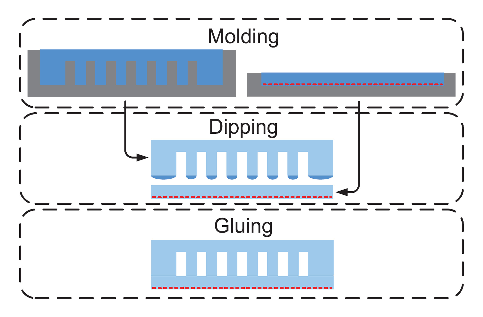
\includegraphics[width=3in]{figures/relatedwork/fabrication.eps}
  \caption[Soft lithography fabrication process.]{Soft lithography fabrication process for soft fluidic elastomer robots. Reproduced with permission from \citet{onal2012modular}.}\label{fig:RW fabrication}
\end{figure}

\subsection{Soft Locomotory Robots}
\label{subsec:RW Land}
In the past years, soft roboticists have made many notable low durometer rubber robots intended for land and water locomotion.
For example, rolling belts have been produced by \citet{correll2010soft} and \citet{marchese2011soft}.
\citet{trimmer2006caterpillar} and \citet{umedachi2013highly} emulated the peristaltic locomotion of caterpillars. \citet{shepherd2011multigait} developed a multi-gait walking robot, and \citet{shepherd2013using} developed a jumping robot powered by combustion.
However, a limitation of the aforementioned locomotory robots is that they require an electrical and/or pneumatic tether.
Soft actuation systems, especially fluidic actuation systems, typically require significant supporting hardware and often limit soft locomotory robots from being self-contained.
That said, there are a few examples of untethered soft robots:
\citet{onal2011soft} created a rolling robot, \citet{onal2013autonomous} emulated the serpentine locomotion of snakes, and \cite{tolley2014resilient} developed a quadrupedal walking robot; these are all soft-bodied fluidic elastomer systems.
\citet{seok2010peristaltic} realize peristaltic locomotion with a self-contained SMA-based inchworm.
However, a limitation of all these untethered soft platforms is that performance is severely limited with respect to their rigid-bodied counterparts, and this limitation is due to the constraints imposed by bringing onboard all supporting hardware.
More specifically, they all exhibit locomotory speeds of between 0.008 and 0.07 body lengths per second.
Recently, \citet{marchese2014autonomous} developed an autonomous soft robotic fish that can perform escape maneuvers with speeds up to 0.4 body lengths per second. \citet{katzschmann2014hydraulic} presented a soft fish that can swim in 3D for prolonged periods of time and powers its FEA tail hydraulically.

\subsection[Soft Continuum Manipulators]{Soft Continuum Manipulators\footnote{\hl{This subsection also appears in the author's related work} \citet{marchese2015design}.}}
Recently, continuum manipulators composed from soft elastic material have been developed.
These soft rubber manipulators can be categorized under two primary morphologies.
The first morphology-type are tendon driven manipulators consisting of variable length tendons, typically cables or shape memory alloy wire, embedded within and anchored to portions of a soft silicone rubber arm.
For example, previous work on soft bio-inspired octopus-like arms developed by \citet{calisti2010study} used tendons and demonstrated capabilities like grasping and locomotion \citep{laschi2012soft, calisti2011octopus}.
Also, \citet{wang2013visual} developed a cable driven soft rubber arm consisting of one large actuated segment that bends bi-directionally.
Lastly, \citet{mcevoy14shape} and \citet{mcevoy2014thermoplastic} used a programmable stiffness spine in conjunction with tendons to achieve shape change in a soft rubber arm.
The second morphology uses fluidic elastomer actuators (see Section~\ref{subsubsec:RW FEA}) distributed among the manipulator's soft body segments.
The primary advantages of using fluidic actuation for soft continuum manipulators is that this energy transmission system: (i) can be lightweight making for easy integration into distal locations of the body, (ii) conforms to the time varying shape of the manipulator, and (iii) does not require rigid components to implement.
There are several examples of soft fluidic grippers described in recent literature.
\citet{deimel2013compliant} developed a pneumatically actuated three-fingered hand made of fiber reinforced silicone that is mounted to a hard industrial robot and capable of robust grasping.
More recently, they have used similar fiber reinforced actuation technology to develop an anthropomorphic soft pneumatic hand capable of dexterous grasps \citep{deimel2014novel}.
Additionally, we have previously shown planar manipulation is possible with an entirely soft robot. That is, a six-segment planar fluidic elastomer robot can be precisely positioned using a closed-loop kinematic controller \citep{marchese2014design, marchese2014whole, katzschmann2015autonomous}.
\citet{ilievski2011soft} created a pneumatic starfish-like gripper composed of FEAs and demonstrated it grasping an egg.
\citet{Stokes2014hybrid} used an FEA-based elastomer quadrupedal robot to grasp objects in a hard-soft hybrid robotic platform.
A puncture resistant soft pneumatic gripper is developed in \citet{shepherd2013soft}.
An alternative to positive pressure actuated soft grippers is the robotic gripper based on the jamming of granular material developed in \citet{brown2010universal}.
Another relevant piece of work is the manually operated 3D elastomer tentacles developed by \citet{martinez2013robotic} containing 9 pneumatic crescent-shaped channels embedded within 3 body segments.



\section{Actuators}
\label{sec:Actuators}
In this section we detail the design and fabrication of three soft fluidic elastomer body segments.
%
The primary design constraint is that the actuated body segments should be composed almost entirely from soft materials.
%
The primary functional specification is that these actuated segments should integrate into an autonomous robotic systems.
%
That is, they should be capable of performing tasks such as trajectory-following in free space, moving dexterously through confined spaces, and/or grasping and placing objects, all without human intervention.

\subsection{Operating Principles}
\label{subsec:Actuators, Operating Principles}
Despite the variability in fluidic elastomer manipulator morphologies, their fundamental operating principles are universal.
This section provides an overview of these operating principles.
Generally, each segment of a fluidic elastomer manipulator bends and this bending is due to material strain.
Figure~\ref{fig:ElastomerBending} illustrates how unidirectional bending arises from material strain.
Consider a block of elastomer where the edges of the top and bottom surfaces have equal lengths, $L_0$.
If the top surface is strained such that its new edge length is $L_0$ + $\Delta L$, but the bottom of this block remains unextended, then the elastomer will bend.
Bending is the basic motion primitive of the fluidic elastomer manipulator.
\begin{figure}[htb]
\centering
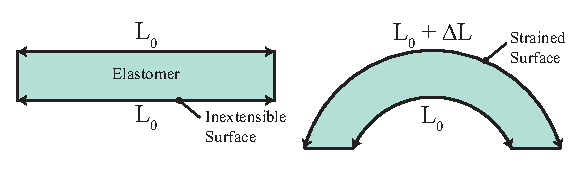
\includegraphics[width=0.85\columnwidth]{figures/actuators/ElastomerBending}
\caption[Operating principle of a bending elastomer segment.]{Operating principle of a bending elastomer segment. One surface of the elastomer is strained while the opposite side remains unextended. The difference in length produces bending.}
\label{fig:ElastomerBending}
\end{figure}

In order to generate strain within the elastomer, this class of manipulators uses pressurized fluids.
Essentially, expandable, fluid-filled chambers are embedded within the elastomer.
When these chambers are pressurized, the entrapped fluid generates stress in the material causing the material to strain.
This concept is illustrated in Figure~\ref{fig:FluidicPower}A and Figure~\ref{fig:FluidicPower}B.
Here, the entrapped fluid is shown in yellow and its pressure is $p_c$.
In order to express the relationship between fluid pressure and elastomer deformation, we can use a one-dimensional simplification of an iterative model presented in \citet{marchese2015design}.
Let $\bar{h}$ and $\bar{t}$ be the initial undeformed diameter and wall thickness of a cylindrical elastomer channel, and let $\hat{h}$ and $\hat{t}$ represent the deformed diameter and wall thickness.
Algorithm~\ref{alg:SimpleModel} expresses how the channel's diameter grows as a function of pressure.
Stresses are successively updated based on deformed channel dimensions.
Here, $\Delta \mathbf{p}_{c}$ is a vector of all consecutive incremental pressure increases until the maximum channel pressure $p_c^{\text{max}}$ is reached.
The stress and strain in the elastomer are represented by $\sigma$ and $\epsilon$, respectively.
The procedure \texttt{strainLookUp()} provides a nonlinear mapping from stress to strain.
\begin{algorithm}[htb]
\footnotesize
  \DontPrintSemicolon
  \SetAlgoLined
  \caption{Iterative Channel Deformation}
  \label{alg:SimpleModel}
  \KwIn{$\bar{t}$, $\bar{h}$, $\Delta \mathbf{p}_{c}$, $p_c^{\text{max}}$}
  $\hat{h} \gets \bar{h}$. \;
  $\hat{t} \gets \bar{t}$. \;
  $\bar{c} \gets \pi \, \left(\frac{\bar{t}}{2} + \bar{h} + \frac{\bar{t}}{2}\right)$. \;
  $p_c \gets p_{\text{atm}}$. \;
  $i \gets 0$. \;
  \Repeat{$p_c \geq p_c^{\text{max}}$}
  {
     $\sigma \gets p_c \frac{\hat{h}}{2 \,\hat{t}}$. \;
     $\epsilon \gets \texttt{strainLookUp}(\sigma)$. \;
     $\hat{c} \gets \bar{c}\left( 1 + \epsilon \right)$. \;
     $\hat{h}, \hat{t} \gets \texttt{solve}\left\{
	\begin{array}{l}
       \text{\textbf{Circumferential Strain:}} \\
       \hat{h} = \frac{\hat{c}}{\pi} - \hat{t} \\
       \text{\textbf{Conservation of Material Volume:}} \\
       \pi \left[ \left( \frac{\hat{h}}{2} + \hat{t}\right)^2 - \frac{\hat{h}^2}{4} \right]= \pi \left[\left( \frac{\bar{h}}{2} + \bar{t}\right)^2 - \frac{\bar{h}^2}{4}\right]
     \end{array}
     \right\} $. \;
     $p_c \gets p_c + \Delta p_{c,i}$. \;
     $i++$
   }
\normalsize
\end{algorithm}

\begin{figure}[htb]
\centering
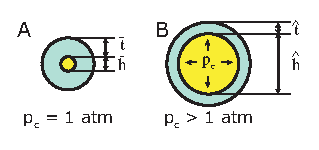
\includegraphics[width=2.0in]{figures/actuators/FluidicPower.eps}
\caption[Operative principle of producing material strain through fluidic power.]{Operative principle of producing material strain through fluidic power. (\textbf{A}) Fluid, shown in yellow, is entrapped in an elastomer channel. (\textbf{B}) When the fluid is pressurized, stress and therefore strain are generated in the material. }\label{fig:FluidicPower}
\end{figure}


\subsection{Actuator Morphologies}
\label{subsec:Actuators, Actuator Morphologies}
This section provides an in-depth look at three separate soft elastomer body segments actuated using pressurized fluids.
%
We use a defining structural feature to refer to each of the presented segment morphologies, those are (i) ribbed, (ii) cylindrical, and (iii) pleated.
%
In Section \ref{sec:Manipulators}, these segments are combined serially to form multi-body manipulators.
%
Although similar in material composition and function, differences in internal and external structure and form lead to several distinct difference between the three presented morphologies.
%
First, we present each morphology, examining the structural differences.
%
Then, we provide a comparative characterization of the segments, highlighting salient performance characteristics.

\subsubsection{Ribbed Segment}
\label{subsubsec:Actuators, Actuator Morphologies, Ribbed}
The ribbed fluidic elastomer actuator with its multiple rectangular channels was first implemented and characterized in \citet{correll2010soft} followed by \citet{onal2011soft, onal2013autonomous}.
%
Joining two fluidic elastomer actuators in an agonist-antagonist pairing provides bidirectional bending.
%
This actuator type provided the fundamental segment-level structure of the manipulator developed in \citet{marchese2014design}.
%
We refer to this three layer composite here as a ribbed segment.
%
That is, two actuator layers are combined in a pair, but separated by an inextensible constraint layer.
%
An implementation of this segment morphology is shown in both a neutral (Fig.~\ref{fig:ribbed design}A) and bent state (Fig.~\ref{fig:ribbed design}B).
%
Bending is produced through the pressurization of agonist fluidic channels (Fig.~\ref{fig:ribbed design}b) that are embedded within the actuated layers (Fig.~\ref{fig:ribbed design}, layers 1 and 3).
%
The structure of the actuated layers is cast from soft elastomer (Fig.~\ref{fig:ribbed design}a).
%
When pressurized, the agonist fluidic channels expand and strain the elastomer.
%
This deformation is transferred into bending by means of an inextensible but flexible constraint (Fig.~\ref{fig:ribbed design}c) embedded within the center layer (Fig.~\ref{fig:ribbed design}, layer 2).
%
Ribs located between channels (Fig.~\ref{fig:ribbed design}e) mitigate strain normal to the inextensible neutral axis.
%
At the segment level, \citet{marchese2014design} extended the ribbed segment design to make it suitable for inclusion in a multi-segment manipulator.
%
Specifically, fluidic supply channels (Fig.~\ref{fig:ribbed design}d) were introduced on either side of the inextensible constraint and embedded within the center layer.
%
Each segment accommodates multiple, parallel supply channels, two for each body segment within the manipulator.
%
For a detailed model of how a ribbed segment deforms under fluidic pressure input, please refer to \citet{marchese2014autonomous}. %why not adding it here?
%
It is important to note that this simplifying static model assumes that ribbed channels deform purely by extending their side and top walls, and that these wall stresses are based on initial channel geometry.
%
In reality, as is shown here in Algorithm~\ref{alg:SimpleModel}, wall stresses change as a function of the deformed geometry.
If needed, Algorithm \ref{alg:SimpleModel} can be used to augment the ribbed model in \citet{marchese2014autonomous}.

\textbf{Pros}: The primary benefits of this morphology in relation to alternatives presented in this section are: (1) Ribs between channels mitigate strain normal to the neutral axis. (2) Smaller changes in input fluid energy produce equivalent bending, and thus for a fixed fluid input, this segment exhibits the highest maximum curvature.

\textbf{Cons}: The primary disadvantages of this morphology in relation to alternatives presented in this section are: (1) The three layer structure is prone to delamination and rupture under high strain. (2) Manufacturing this rectangular, layered structure is challenging because all transmission lines must be embedded within the thin constraint layer.

\begin{figure}[htb]
\centering
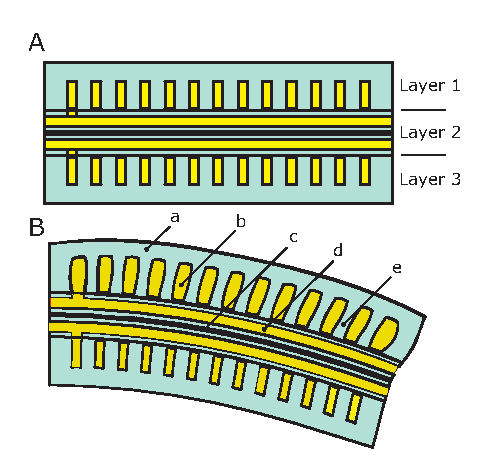
\includegraphics[width=2.9in]{Figures/actuators/ribbed_design.eps}
\caption[A conceptual representation of the ribbed segment morphology]{A conceptual representation of the ribbed segment morphology. The segment is composed of three layers produced from soft elastomer (a), embedded fluidic channels (b), inextensible, but flexible constraint (c), embedded fluid transmission lines (d), and ribbed structures (e). (\textbf{A}) The segment in an unactuated, or neutral state. (\textbf{B}) The segment in an actuated state where fluid within the agonist channel group is pressurized producing bending about the inextensible axis.} \label{fig:ribbed design}
\end{figure}

\subsubsection{Cylindrical Segment}
\label{subsubsec:Actuators, Actuator Morphologies, Cylindrical}
The cylindrical fluidic elastomer segment is an alternative to the ribbed design.
%
This design was first presented by the authors in \citet{marchese2014whole}.
%
Design inspiration was drawn from the soft rubber tentacles developed by \citet{martinez2013robotic} which use embedded crescent-shaped channels in a similar two-layer rubber construction.
%
Although the cylindrical segment morphology is notably different from the ribbed segment, the fundamental operating principles are the same.
%
In the cylindrical morphology (Fig.~\ref{fig:cylindrical_design}A and B), we transition from a rectangular, planar-layered composite to a cylindrical, concentric-layered composite.
%
Specifically, the segment consists of three concentric layers: (i) an outer soft layer (Fig.~\ref{fig:cylindrical_design}b, \emph{transparent}), (ii) a slightly stiffer inner layer (Fig.~\ref{fig:cylindrical_design}d, \emph{green}), and (iii) a hollow core that accommodates a bundle of fluid transmission lines (Fig.~\ref{fig:cylindrical_design}f, \emph{white}).
%
Two fluid-filled, and cylindrically-shaped channels are embedded laterally within the outermost layer (Fig.~\ref{fig:cylindrical_design}c).
%
These channels interface with the transmission lines by means of a stiffer rubber inlet piece (Fig.~\ref{fig:cylindrical_design}a, \emph{brown}).
%
When pressurized, the entrapped fluid deforms the embedded channel both circumferentially and longitudinally (Fig.~\ref{fig:cylindrical_design}B).
%
Specific to this morphology, the inner tube-like layer composed of slightly stiffer rubber serves as an inextensible constraint, transforming channel deformation into segment bending.

%%structural impendance two sentence

\textbf{Pros}: The primary benefits of this morphology in relation to alternatives presented in this section are: (1) Entirely composed of rubber, the resiliency and the durability of the actuator are increased. (2) The two cylindrical channels make this segment the simplest to fabricate. (3) Embedded fluidic channels are not at the interface between fabrication layers, making this morphology robust against delamination under high pressures.

\textbf{Cons}: The primary disadvantages of this morphology in relation to alternatives presented in this section are: (1) The simple channel design exhibits high circumferential strain. Compared to the ribbed morphology, more fluid energy is required to produce curvature. (2) When the segment bends, an increased volume of rubber on the antagonist side of the actuator has to be compressed. This inhibits a high curvature.

\begin{figure}[htb]
\centering
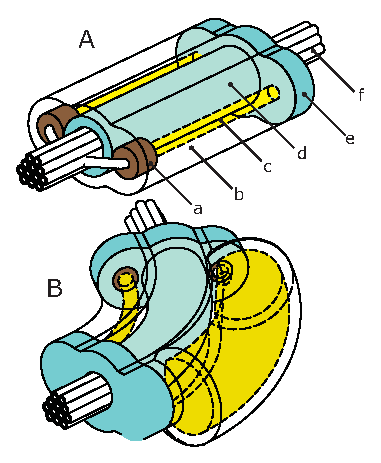
\includegraphics[width=2.9in]{Figures/actuators/cylindrical_design.eps}
\caption[A conceptual representation of the cylindrical segment morphology.]{A conceptual representation of the cylindrical segment morphology. The segment consists of a soft silicone rubber outer layer (b, \emph{transparent}), a slightly stiffer silicone inner layer (d, \emph{cyan}), crush resistant silicone inlets (a, brown), expanding embedded fluidic channels (c, \emph{yellow}), and an internal tubing bundle (f, \emph{white}). The segment terminates in soft endplates (e). (\textbf{A}) A depiction of the segment in an unactuated state. (\textbf{B}) A depiction of the body segment in an actuated state where the expansion of the pressurized fluidic channel is schematically represented.
}\label{fig:cylindrical_design}
\end{figure}

\subsubsection{Pleated Segment}
\label{subsubsec:Actuators, Actuator Morphologies, Pleated}
The pleated channel design is detailed in Figure~\ref{fig:pleated_design} and consists of evenly spaced, discrete elastomer sections (Fig.~\ref{fig:pleated_design}d), which are separated by gaps (Fig.~\ref{fig:pleated_design}c).
%
Embedded within each elastomer section is a hollow channel (Fig.~\ref{fig:pleated_design}e).
%
Cut views of the un-actuated and actuated states are shown in Figure~\ref{fig:pleated_design}A and Figure~\ref{fig:pleated_design}B, respectively.
%
This design approach draws inspiration for its pleats from the soft pneumatic gloves developed by \citet{polygerinos2013towards} and its homogeneous body design is inspired from the tail design of a soft robotic fish developed by \citet{katzschmann2014hydraulic}.
%
The hollow channel within each pleat are connected by a center channel and are accessible through a front inlet (Fig.~\ref{fig:pleated_design}a).
%
When fluid within these channels is pressurized (Fig.~\ref{fig:pleated_design}, \emph{yellow}), an individual pleat undergoes a balloon-like expansion of the thin exterior skin both normal and parallel to the neutral axis.
%
Similar to the uniform channel design, a stiffer silicone layer (Fig.~\ref{fig:pleated_design}, \emph{blue}) serves as an almost inextensible constraint layer.
%
The sum of the balloon-like expanding motions leads to bending of the less extensible center constraint layer.

\textbf{Pros}: The primary benefits of this morphology in relation to alternatives presented in this section are: (1) A unidirectional pleated actuator is capable of bending to higher curvatures than the ribbed or cylindrical morphology.
(2) A bidirectional pleated segment is capable of exerting higher maximum forces because of its ability to accommodate the largest energy input.
(3) Using a lost-wax casting approach, the \emph{cyan} portion of this segment can be cured in a single step, avoiding seams that are prone to delamination.

\textbf{Cons}: The primary disadvantages of this morphology in relation to alternatives presented in this section are: (1) The morphology is more complex to manufacture, because a wax core has to be produced and after curing, it has to be melted out again. (2) The implementation of this morphology requires the most fluid energy to actuate it to appreciable tip force. This might very well be, because the implementation is larger in size and a higher shore hardness elastomer is used, when compared to the other implementations.

\begin{figure}[htb]
\centering
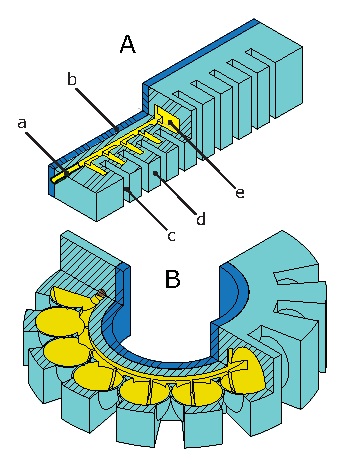
\includegraphics[width=2.9in]{Figures/actuators/pleated_design.eps}
\caption[A conceptual representation of the pleated segment morphology.]{A conceptual representation of the pleated segment morphology. The design consists of a channel inlet (a), an almost inextensible constraint layer (b), uniform pleats (d) separated by even gaps (c), and internal channels within each pleat (e). (\textbf{A}) depicts the segment in an unactuated state and (\textbf{B}) shows the segment in an actuated and therefore bent state. The expansion of the pressurized channels are schematically represented.}\label{fig:pleated_design}
\end{figure}

\subsubsection{Comparative Characterization}
\label{subsubsec:Actuators, Actuator Morphologies, Characterization}
To characterize the actuated segments, we first perform bending tests to experimentally determine the relationship between the segment's neutral axis curvature $\kappa$, internal channel pressure $p_c$, and supplied volume $\mathbb{V}_s$ for each morphology.
%
In these experiments, the base of each segment is grounded securely in a fixture and the segment's tip is supported vertically with a ball transfer. %removed: ", if necessary." <-because this seems like vague statement
%
Then, the segment's agonist channel is incrementally filled under closed-loop volume control via the displacement of a fluidic drive cylinder; please refer to Section~\ref{sec:Power}.
%
After each incremental fill, we allow pressure within the cylinder and within the actuated channel to equalize before measurements of the channel's pressure and the segment's curvature are taken.
%
Curvature is assumed to be constant along the length of the segment and is uniquely defined by measuring the cartesian locations of the base and the tip of the segment.
%; refer to Section~\ref{subsec:Kinematic Modeling, SSIK}.
%
Since this is a quasi-static process, fluid pressure and supply volume measurements can be used to determine the elastic potential fluid energy input into the actuation system, which consists of the elastomer segment and the internal compressible transmission fluid.
The potential energy is calculated by
\begin{equation}\label{eqn:energy}
    V_{Elastic} = \int_0^{\mathbb{V}_c} p_c\left( \mathbb{V} \right) \, \text{d} \mathbb{V}.
\end{equation}
%
Additionally, a blocking force test is performed in order to understand the variability in tip force output between segment morphologies.
%
Again, a similar experimental procedure is used as for the curvature measurements; however, during blocking force experiments a plate attached via a force transducer to ground is mounted in contact with the segment's tip, orthogonal to the bending plane.
%
This effectively measures the force required to block the actuator from bending.
%
\begin{figure*}[htb]
        \centering
        \begin{subfigure}[b]{\columnwidth}
            \centering
            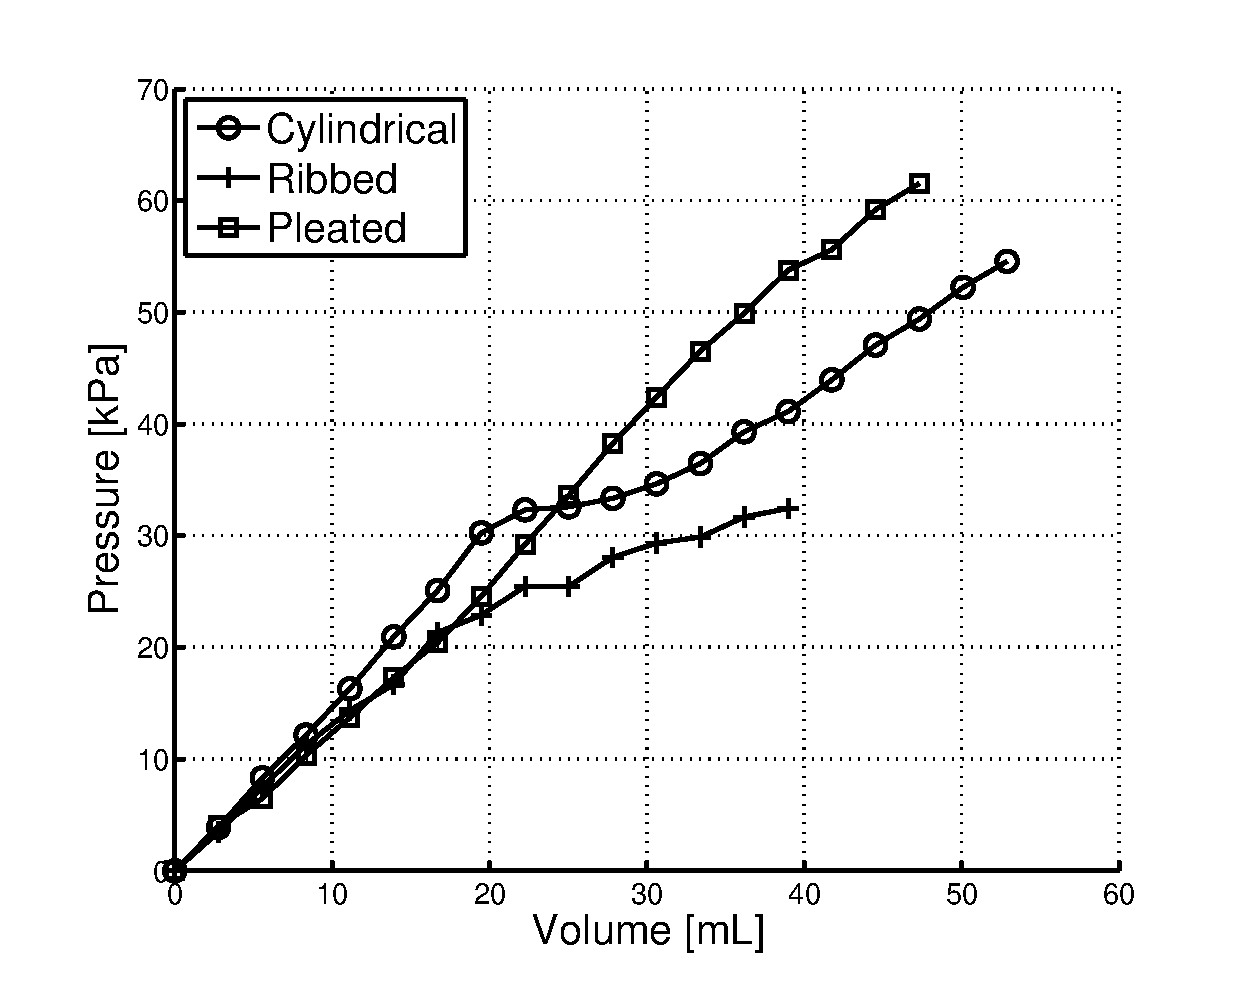
\includegraphics[width=0.95\columnwidth]{figures/actuators/morphologiescharacterization/PressureVsVolume.eps}
            \caption{}
            \label{fig:Characterization_PressureVsVolume}
        \end{subfigure}
        \begin{subfigure}[b]{\columnwidth}
            \centering
            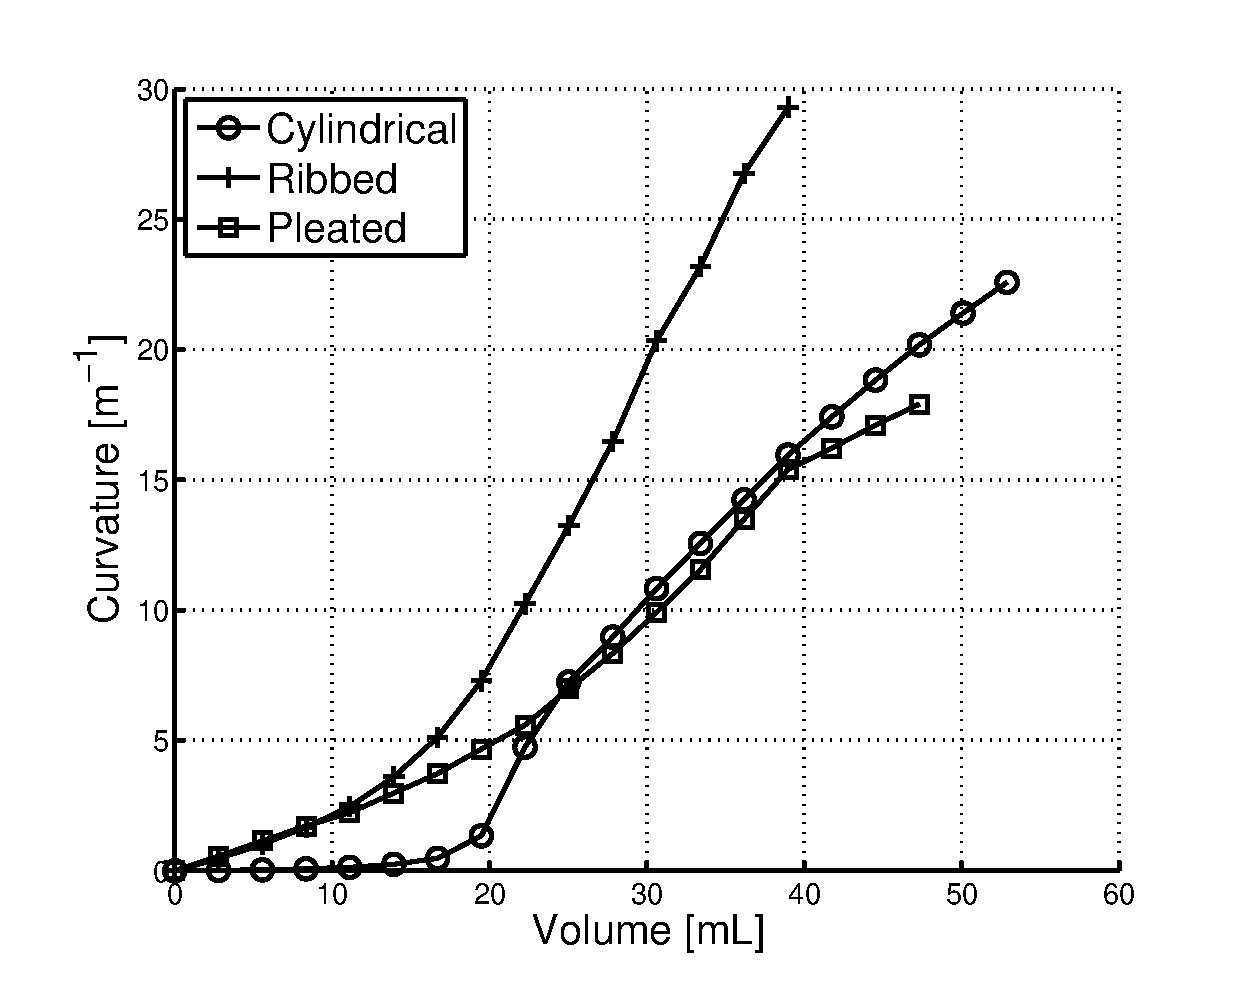
\includegraphics[width=0.95\columnwidth]{figures/actuators/morphologiescharacterization/CurvatureVsVolume.eps}
            \caption{}
            \label{fig:Characterization_CurvatureVsVolume}
        \end{subfigure} \\
                \begin{subfigure}[b]{\columnwidth}
            \centering
            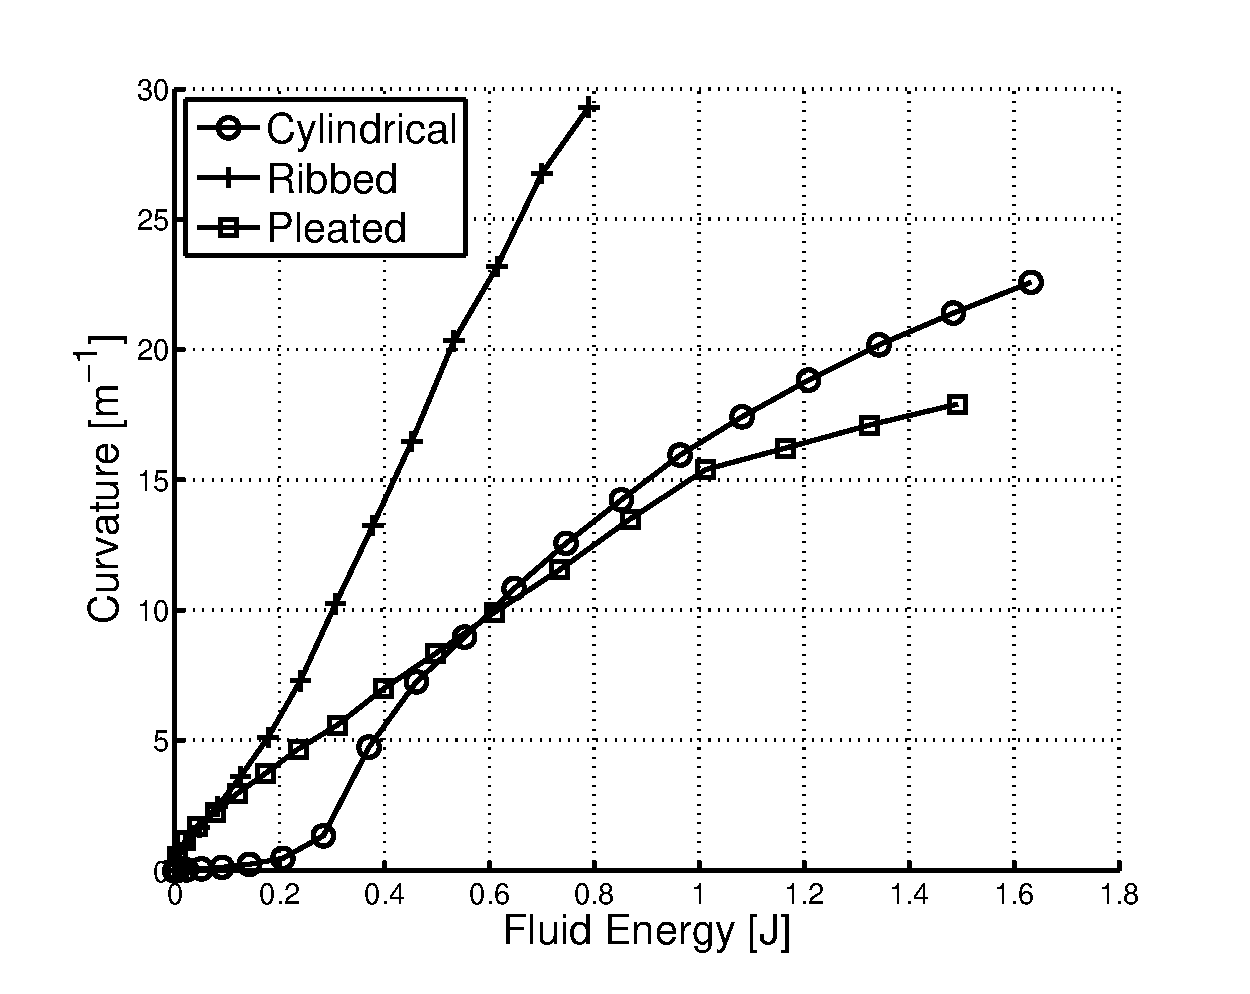
\includegraphics[width=0.95\columnwidth]{figures/actuators/morphologiescharacterization/CurvatureVsEnergy.eps}
            \caption{}
            \label{fig:Characterization_CurvatureVsEnergy}
        \end{subfigure}
        \begin{subfigure}[b]{\columnwidth}
            \centering
            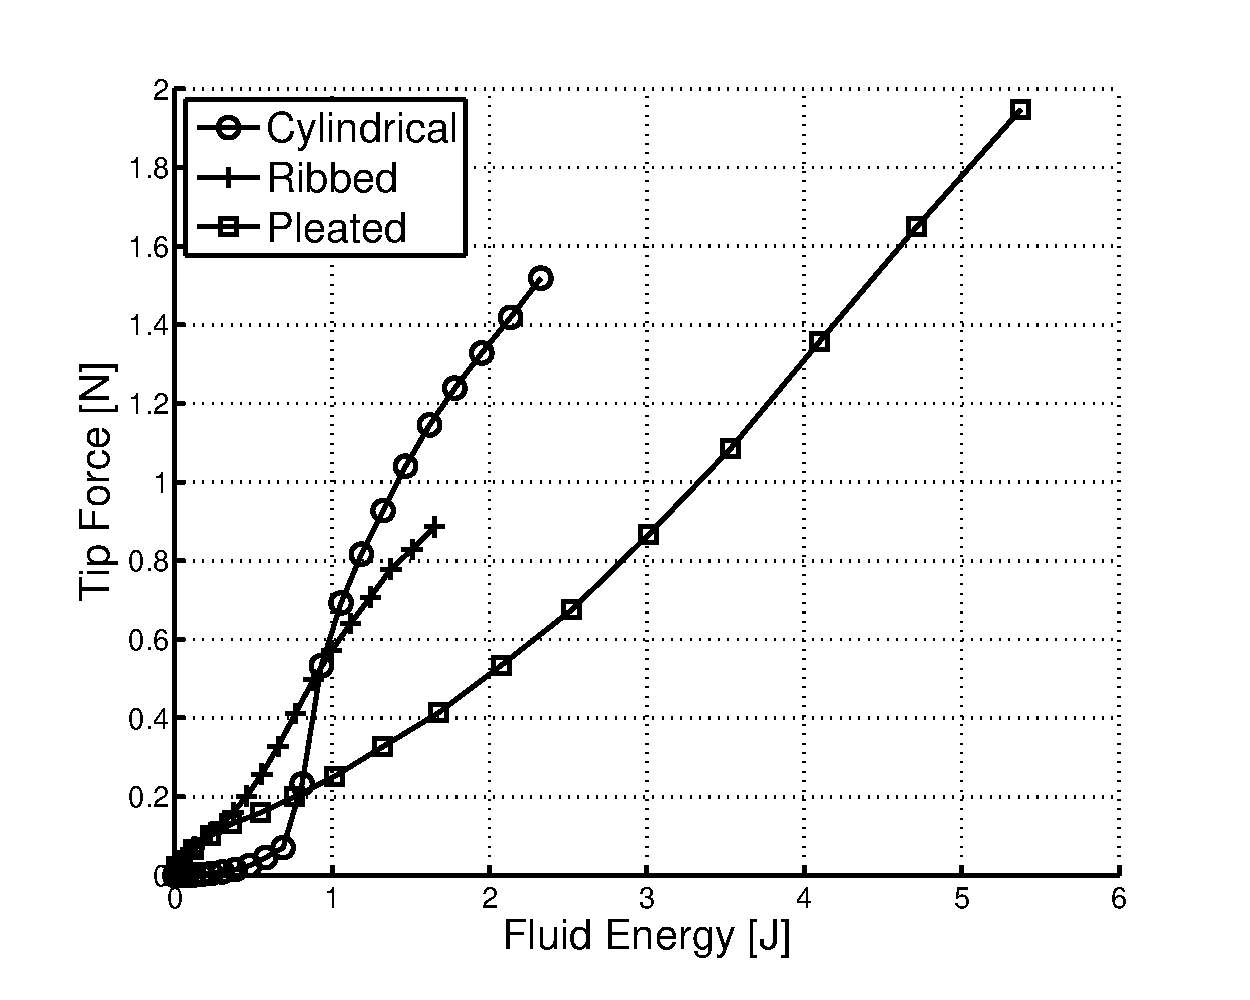
\includegraphics[width=0.95\columnwidth]{figures/actuators/morphologiescharacterization/ForceVsEnergy.eps}
            \caption{}
            \label{fig:Characterization_ForceVsEnergy}
        \end{subfigure}
        \caption[Experimental characterizations of three actuated segment morphologies.]{Experimental characterizations of three actuated segment morphologies performed by filling each actuator by means of controlled volumetric displacements and measuring internal pressure, neutral axis curvature under a constant-curvature assumption, and blocking force.}\label{fig:actuator_characterization}
\end{figure*}

Figure~\ref{fig:actuator_characterization} details the results of these characterization experiments, based on which we can make several observations.
%
First, the pleated morphology is generally the stiffest, followed by the cylindrical, and then the ribbed, whereas stiffness is defined as $\frac{\partial p_c}{\partial \mathbb{V}_c}$ (Fig.~\ref{fig:Characterization_PressureVsVolume}).
%
Second, the cylindrical morphology has a salient curvature nonlinearity (Fig.~\ref{fig:Characterization_CurvatureVsVolume}).
%
More specifically, small volumetric fluid changes for less than $15\,$mL provide little control authority over curvature; however, above $25\,$mL displacements, the control authority is strong and the curvature-volume relationship is approximately linear.
%
Third, the ribbed morphology requires the least amount of fluid energy to produce a given curvature (Fig.~\ref{fig:Characterization_CurvatureVsEnergy}).
%
This means that the ribbed segment requires approximately half the amount of fluid energy needed by the cylindrical and pleated segments to produce a significant bending (greater than $7\,\text{m}^{-1}$).
%
Lastly, the pleated segment generally requires more fluid energy than both the ribbed and cylindrical morphologies to produce a given tip force.
%
However, the pleated segment can accommodate significantly higher input energies and therefore can reach the highest maximum tip force.




\section{Fabrication}
\label{sec:Fabrication}
Three distinct fabrication techniques for soft actuators are show-cased with the help of the previously described multi-segment arm designs.
Table~\ref{tab:MachineTools} contains the superscript references to machine tools and materials used.

	
\subsection{Soft Lithography with Heterogenous Embeddings}
\label{subsec:Fabrication, Soft Lithography with Heterogenous Embeddings}
Soft lithography with heterogeneous embedding as a fabrication technique is shown for a ribbed actuator morphology. The ribbed manipulator is composed of six actuator segments and is fabricated from various soft and semi-soft materials.
Seven constraint supports (Fig.~\ref{fig:ribbed fab process}d) are 3D printed$^1$ and placed into a constraint layer mold (Fig.~\ref{fig:ribbed fab process}f), which is also 3D printed.
The constraint film (Fig.~\ref{fig:ribbed fab process}c) is cut from a thin acetal sheet$^8$ using a laser$^2$ and inserted through the aforementioned supports.
Above and below the constraint film, eight pieces of silicone tubing (Fig.~\ref{fig:ribbed fab process}a) are threaded through the supports.
Silicone rubber$^3$ is then mixed and poured into the constraint layer mold, immersing tubing, film, and supports in a layer of elastomer to create the composite constraint layer (Fig.~\ref{fig:ribbed fab process}g).
The uncured rubber inside the mold is then immediately degassed using a vacuum chamber$^4$.
Once cured, small holes are created in the constraint layer to pierce the embedded tubing at specific locations, allowing each line to independently address a group of fluidic channels.
Elastomer pieces containing channels (Fig.~\ref{fig:ribbed fab process}b) are casted and cured separately using a similar molding technique.
Those cured elastomer pieces (Fig.~\ref{fig:ribbed fab process}b) are then carefully attached to both faces of the constraint layer using a thin layer of silicone rubber.
Lastly, the printed feet (Fig.~\ref{fig:ribbed fab process}e) are attached to the constraint supports (Fig.~\ref{fig:ribbed fab process}d) to create an attachment point for ball transfers (Fig.~\ref{fig:ribbed_manipulator_design}d).
These mechanisms prevent the arm from tipping and help constrain the arm's motion to the X-Y plane.

\begin{figure}[htb]
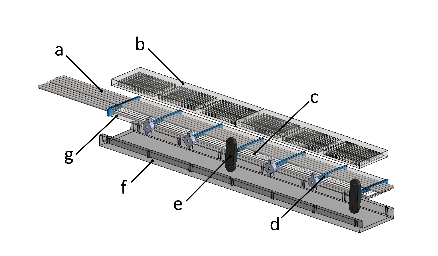
\includegraphics[width=\columnwidth]{figures/fabrication/fab_ribbed_process.eps}
\caption[Fabrication process for a ribbed manipulator morphology]{Fabrication process for a ribbed manipulator morphology: silicone tubing (a), elastomer pieces containing channels (b), constraint film (c), constraint supports (d), feet (e), constraint layer mold (f), and composite constraint layer (g).}
\label{fig:ribbed fab process}
\end{figure}

\subsection{Retractable Pin Casting}
\label{subsec:Fabrication, Retractable Pin Casting}
The cylindrical manipulator is fabricated through a casting process that uses pourable silicone rubber$^{3,5}$ and 3D printed molds$^1$.
Figure~\ref{fig:cylindrical_fab} details this process.

First, each body segment is independently fabricated in steps 1-3 and later these segments are joined serially to form the arm in steps 4 and 5.
To start, a four piece mold is printed.
The mold is then poured in two steps.
In step 1, a low elastic modulus rubber$^3$ is mixed, degassed in a vacuum$^4$, and poured to form the body segment's soft outer layer shown in \emph{white}.
The mold's outer piece, one half of it is shown in \emph{green}, functions to form the segment's exterior.
Metal rods shown in \emph{pink} are inserted into the mold and are held in place by the \emph{orange} bottom piece of the mold.
These rods will form the cavities for the segment's two lateral fluidic actuation channels.

After the outer layer has cured, the \emph{red} rigid sleeve is removed in step 2 from the extruded feature of the \emph{orange} bottom piece of the mold.
This produces a cavity into which a slightly stiffer rubber$^5$ is poured, forming the segment's partially constraining inner layer shown in \emph{cyan}.
The extruded feature of the \emph{orange} bottom piece, shown by its \emph{orange} end tip, functions to produce the segment's hollow interior core.
In step 3, the body segments are removed from their molds and joined to rubber$^5$ endplates shown in \emph{cyan} using silicone adhesive$^6$.
The small \emph{yellow} channel inlets were added on one side of the \emph{pink} metal pins during step 1.
In step 4, soft silicone tubes$^7$ are joined to each embedded channel's inlet.
The resulting bundle of tubes is passed through each segment's hollow interior.
Lastly, in step 5 multiple body segments are attached at their endplates using the same adhesive$^6$.

\begin{figure}[htb]
\centering
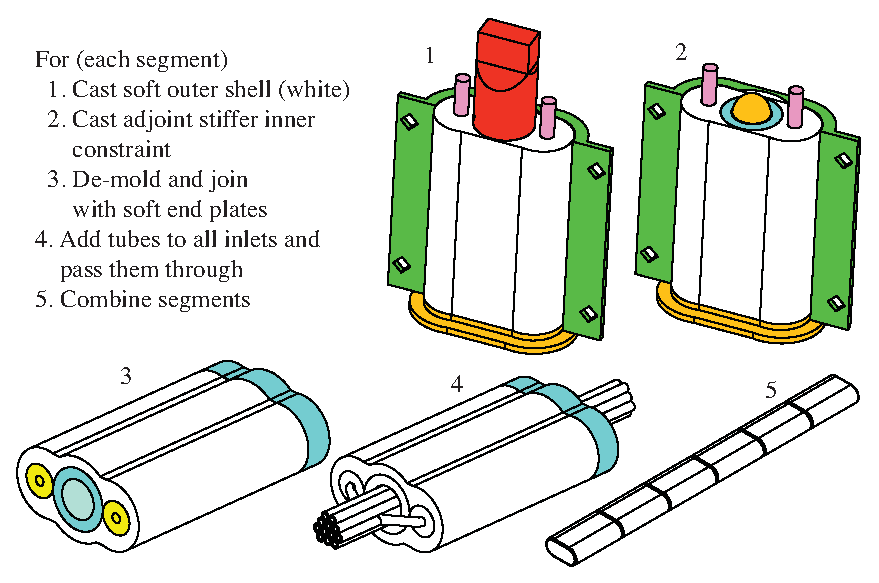
\includegraphics[width=\columnwidth]{figures/fabrication/fab_cylindrical_process.eps}
\caption[Fabrication process for the cylindrical manipulator morphology]{Fabrication process for the cylindrical manipulator morphology: Each body segment is casted using a two step process where the outer soft layer (\textbf{1}) and inner stiffer layer (\textbf{2}) are poured. Once cured, the segments are joined to endplates using silicone adhesive (\textbf{3}). Next, silicone tubing is connected to each embedded channel and the resulting tubing bundle is run inside each segment's hollow interior (\textbf{4}). Lastly, the body segments are serially connected using adhesive to form the manipulator (\textbf{5}).}
\label{fig:cylindrical_fab}
\end{figure}

\subsection{Lost Wax Casting}
\label{subsec:Fabrication, Lost Wax Casting}
Existing soft manipulators are produced through a multi-step lamination process, which produces seams and is easy to delaminate.
This limits their range of applications and lifetime.
By abandoning the need for a lamination process, arbitrary shaped internal channels can be achieved to enable a wider range of applications.
For these reasons, we introduce lost-wax casting as part of the fabrication process for soft actuators.
%The actuated cavities of the soft actuator are achieved by using bees-wax core$^{8}$, pourable silicone rubber$^{2,4,7}$ and 3D printed molds$^1$.
As an example, we fabricate the pleated actuated using the lost-wax approach.
The complete fabrication process for the pleated manipulator consists of eight steps that are depicted in Figure~\ref{fig:pleated_fab} and a final concatenation step.

\begin{figure}[htb]
\centering
   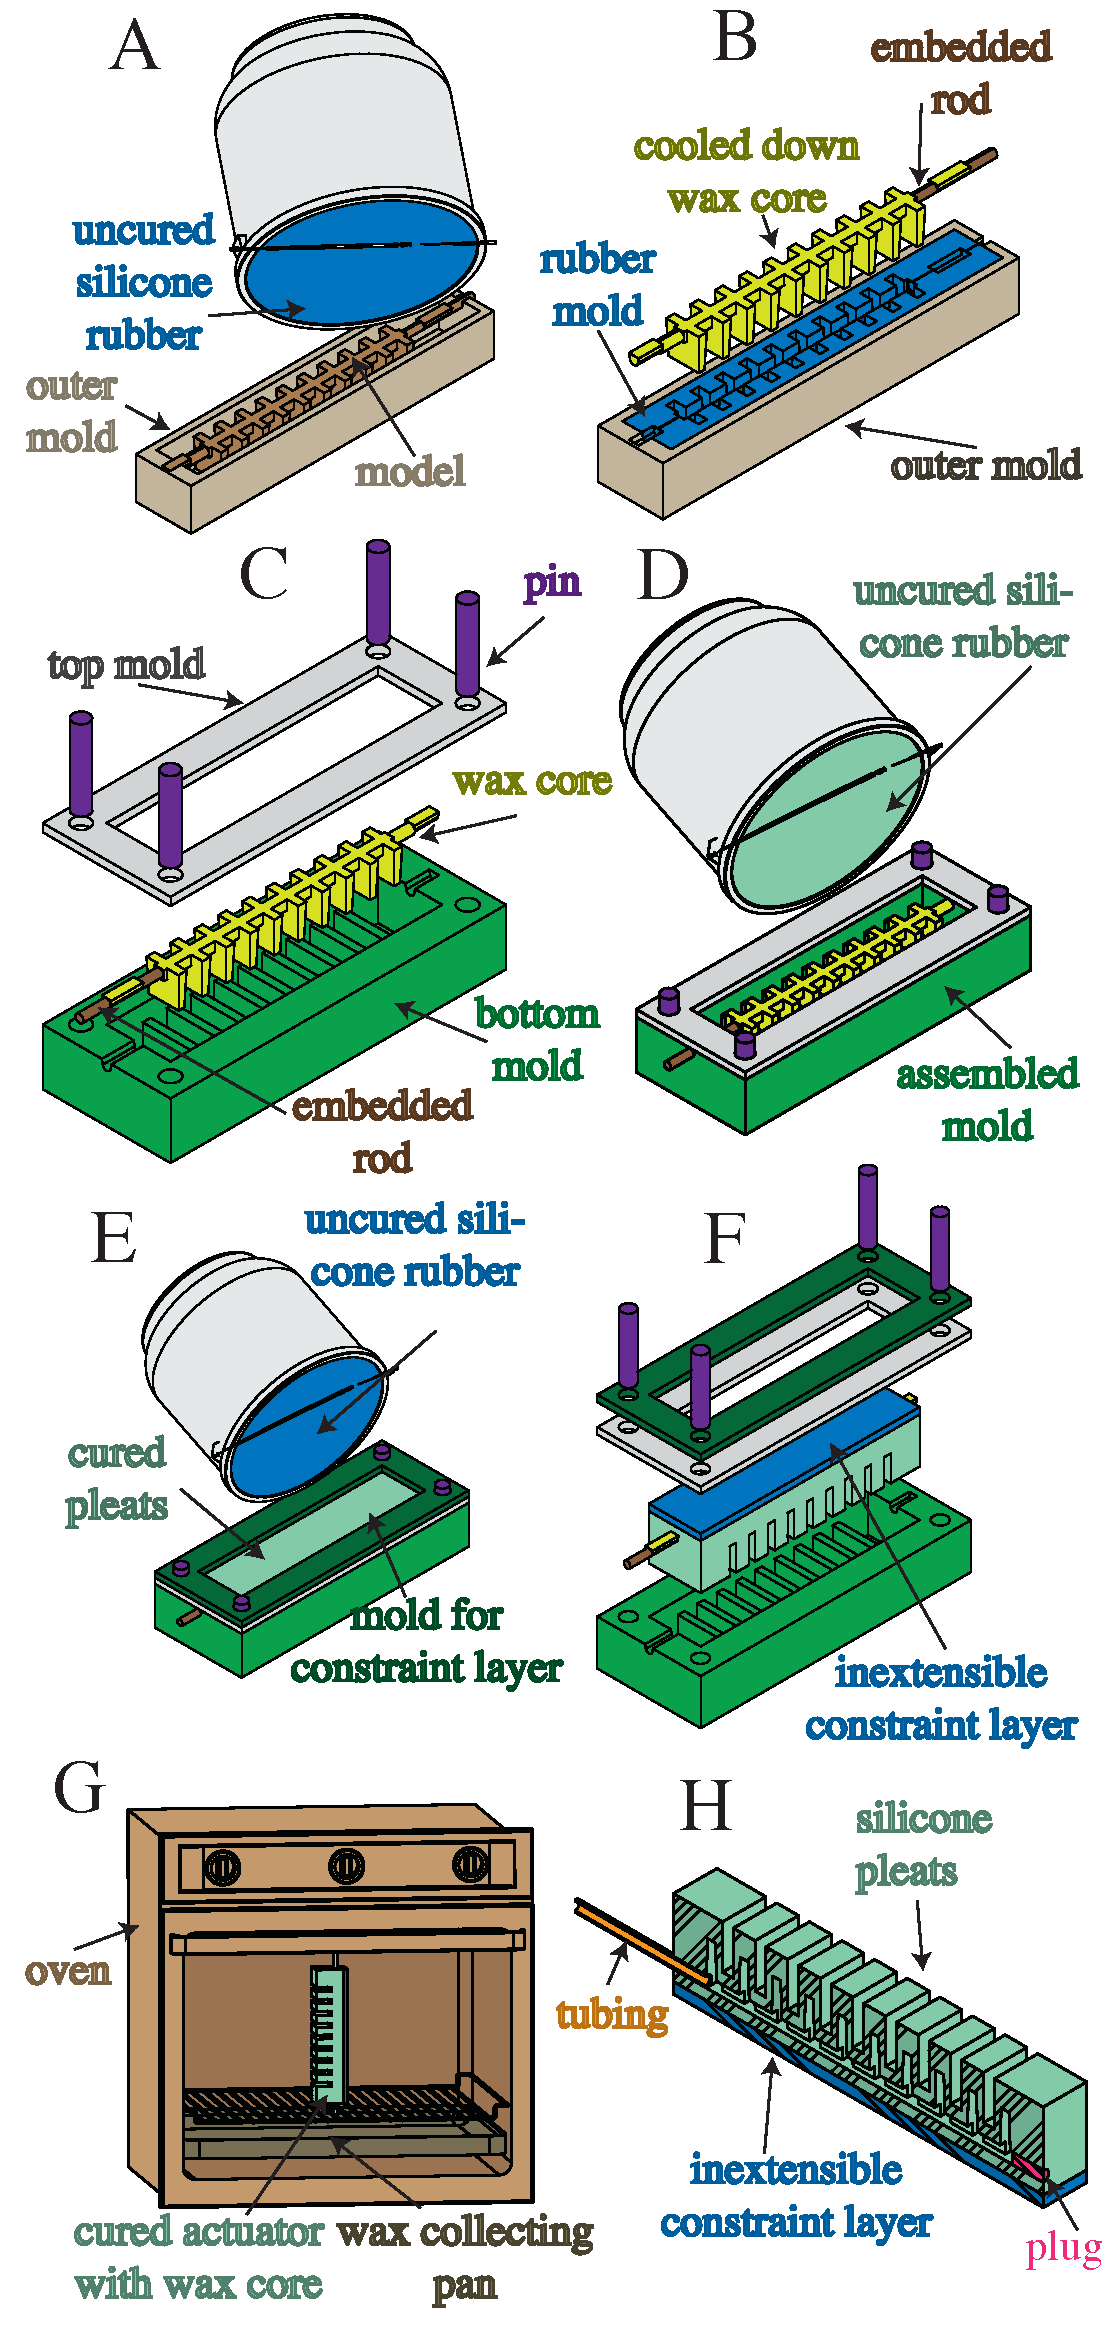
\includegraphics[width=\columnwidth]{figures/fabrication/fab_pleated_process.pdf}
      \caption[Fabrication process for the pleated actuator morphology]{Fabrication process for the pleated actuator morphology: (\textbf{A}) Pour and cure a rubber mold, (\textbf{B}) pour wax core with embedded supportive rod, (\textbf{C}) combine bottom mold, top mold and wax core using pins, (\textbf{D}) pour rubber into assembled mold, (\textbf{E}) pour stiffer rubber on top of the cured actuator to form a constraint layer, (\textbf{F}) remove cured actuator from mold, (\textbf{G}) melt out wax core from the actuator using an oven, and (\textbf{H}) add silicone tubing and plug using silicone sealant.}
      \label{fig:pleated_fab}
\end{figure}

In step (A), harder silicone rubber$^{10}$ is poured into a mold, which contains a 3D printed model of the wax core.
In preparation for step (B), the model is removed and the rubber mold is left inside the outer mold.
Next, a rigid rod or tube, for example made of carbon fiber$^{12}$, is used as a supportive inlay for the wax core.
The rod is laid into the cavity of the rubber mold, supported on both ends by the outer mold.
This ensures that the wax core does not break when removed from the rubber mold.
Mold release spray is applied to the silicone rubber mold to ease the wax core removal process.
The wax$^{11}$ is heated up until it becomes fully liquefied.
The assembly of the rubber mold and the outer mold is heated up for a few minutes to the same temperature as the wax.
Using a syringe, the liquid wax is injected into the assembly.
Within a few minutes, the injected wax will start to solidify and significantly shrink in volume; this is counteracted by injecting more hot wax into the solidifying wax core during the cool down period.
In step (B), the wax core is first allowed to completely cool down, then it is released from the mold.
In step (C), the cooled down wax core is assembled together with the bottom mold, which defines the pleated structure of the actuator.
The mold assembly is aligned with a top mold using pins. This top mold provides additional volume to cover the wax core.
In step (D), low elastic modulus rubber$^3$ is mixed, degassed in a vacuum$^4$, and poured to form the pleats and allowed to cure.
In step (E), stiffer rubber is poured on top of the cured pleats to form a constraint layer.
In step (F), the cured actuator is removed from the mold.
In step (G), most of the wax core is melted out by placing the cured actuator into an oven in an upright position.
After this, remaining wax residues are cooked out in a boiling water bath.
Finally, in step (H) a silicone tube$^9$ and a piece of silicone cord$^13$ get covered with silicone adhesive$^6$ and are inserted into the front and back holes, respectively.

Lastly, the actuator can be used as a unidirectional gripper or as one agonist side segment of a multiple body manipulator, where each segment can be actuated bidirectionally; see Section~\ref{subsec:Manipulators, Pleated}.

\begin{table}[htb]
\caption{Commercially Available Tools and Equipment}
\centering
\begin{tabular}{c l l}
\hline
\hline
\# & Product Name & Company\\
\hline
1 & Fortus 400mc & Stratasys\\
2 & VLS3.50 & Universal Laser Systems\\
3 & Ecoflex 0030 & Smooth-On\\
4 & AL Cube & Abbess Instr. \& Systems\\
5 & Mold Star 15 & Smooth-On\\
6 & Silicone Sealant 732 & Dow Corning\\
7 & PN 51845K52 & McMaster\\
8 & PN 5742T51 & McMaster\\
9 & PN 51845K53 & McMaster\\
10 & Mold Star 30 & Smooth-On\\
11 & Beeswax & Jacquard\\
12 & PN 2153T31& McMaster\\
13 & PN 9808K21& McMaster\\
\hline
\end{tabular}
\label{tab:MachineTools}
\end{table} 

\section{Power}
\label{sec:Power}
Fluidic power sources present many challenges for soft robots.
There are three major ways to characterize these power sources: by transmission fluid, circuit continuity, and portability.

\subsection{Transmission Fluids}
Recently, \citet{wehner2014pneumatic} reviewed existing pneumatic energy sources.
However, in general the actuators detailed in Section~\ref{subsec:Actuators, Actuator Morphologies} can be powered using either pneumatic or hydraulic systems where gases or liquids, respectively, are the transmission fluid.
Pneumatics are advantageous for powering FEAs because they provide a low viscosity power transmission medium.
High flows can be achieved with relatively low driving pressures.
However, gases also introduce compressibility into the power transmission system and these dynamics can be difficult to model (refer to \citet{marchese2015control}) and can produce undesirable time delays.
Hydraulics are advantageous because liquids are relatively incompressible when compared to gases, meaning power can be transferred almost immediately from the power source to the actuators.
However, to achieve comparable volumetric flow rates liquid drive systems often require high driving pressures and/or low impedance (large diameter) power transmission lines because of the increased viscosity of the transmission medium.

\subsection{Circuit Continuity}
Further, the actuators detailed in Section~\ref{subsec:Actuators, Actuator Morphologies} can be powered using either open-circuit or closed-circuit power systems.
Open-circuit power systems exhaust the transmission fluid to the environment, whereas closed-circuit systems recover fluid delivered to the actuators.
open-circuit systems are advantageous because they do not require mechanisms to re-pressurize and return transmission fluid to the supply.
However, they often rely on passively exhausting transmission fluid to ambient/environmental pressure meaning the actuator depressurization is unactuated and a function of the actuator's compliance and the impedance of the the exhaust pathway.
Please refer to \citet{marchese2011soft} and \citet{marchese2014autonomous} for examples of open-circuit power systems.
Closed-circuit systems (see Fig.~\ref{fig:tail_actuation_principle}) are advantageous because the amount of transmission fluid is constant and moved around within the system; this means the power system's fluid medium is not required to match the operating environment (e.g., a soft robot fish powered by pneumatics swimming underwater).
Furthermore, because the volume of transmission fluid is constant the power system can typically vacuum fluid from the actuator under power; meaning the system has control authority over actuator depressurization.
The disadvantage to closed-circuit systems is that they typically require additional plumbing to complete the fluid circuit and supporting hardware like a revisable pump.
Please refer to \cite{marchese2014design, katzschmann2014hydraulic} and \cite{marchese2015design} for examples of closed-circuit power systems.

\subsection{Portability}
The portability of a power source may be of significant interest to a soft roboticist.
For example, locomotory soft robots are typically designed under the constraint of being self-contained, meaning all supporting hardware is located onboard the robot.
Additionally, if the untethered robot is intended for high speed maneuvers, then compressed gas \citep{marchese2014autonomous} or combustion \citep{tolley2014untethered} are viable power alternatives.
However, if prolonged operations are required, then open-circuit pumps \citep{tolley2014resilient, onal2013autonomous} or closed-circuit pumps \citep{katzschmann2014hydraulic} are suitable options.
\begin{figure}[htb]
        \centering
            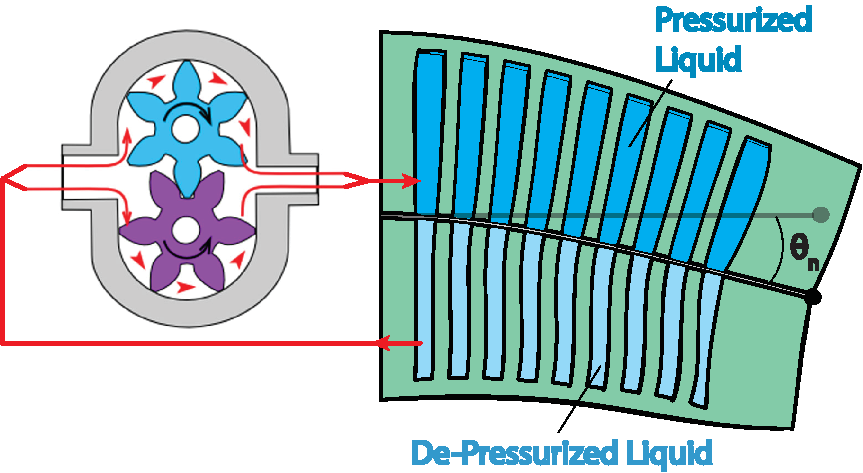
\includegraphics[width=0.85\columnwidth]{figures/power/fish_actuation_principle.pdf}
        \caption[Fish's soft tail actuation principle]{Closed-circuit power system used to drive actuation in the soft hydraulic fish.}
            \label{fig:tail_actuation_principle}
\end{figure}


\section{Locomotion}
\label{sec:Locomotion}
Soft and continuously deformable locomotion systems can be made from fluidic elastomer body segments.
Specifically, in this section we detail how soft robotic fish can be composed by combining the actuated segments that were presented in Section~\ref{subsec:Actuators, Actuator Morphologies} with a portable power system.

\subsection{Pneumatic Fish}
\label{subsec:Locomotion, Pneumatic Fish}
The soft pneumatic fish developed in \cite{marchese2014autonomous} with a ribbed actuator is shown as a complete system in Figure~\ref{fig:pneumaticfish_system} and performing an escape response in Figure~\ref{fig:pneumaticfish_escape}.

\begin{figure}[htb]
        \centering
        \begin{subfigure}[b]{\columnwidth}
            \centering
            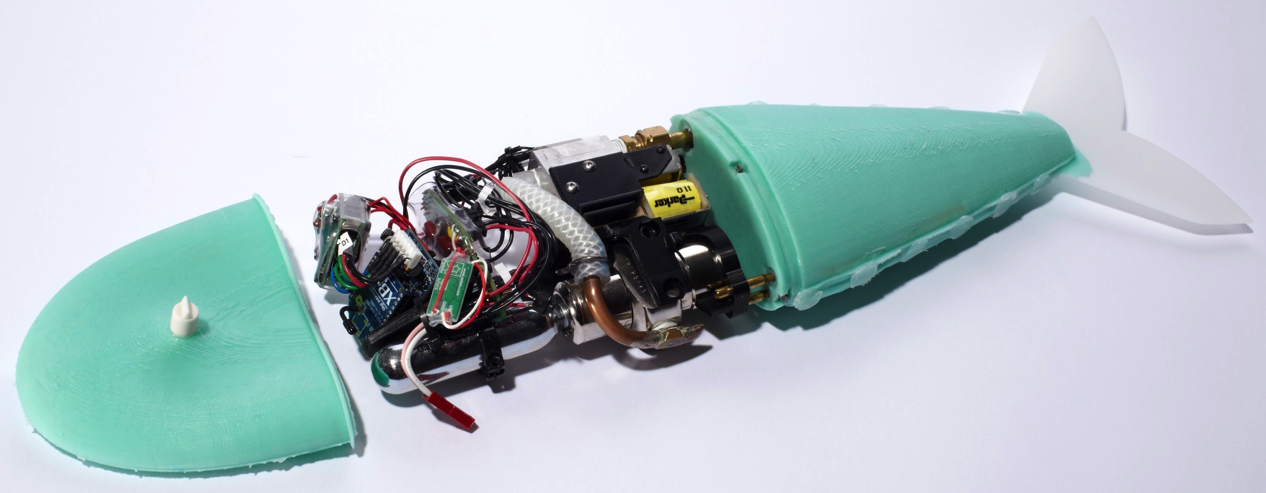
\includegraphics[width=0.9\columnwidth]{Figures/locomotion/pneumaticfish_system.png}
            \caption{}
            \label{fig:pneumaticfish_system}
        \end{subfigure}\\
        \begin{subfigure}[b]{\columnwidth}
            \centering
            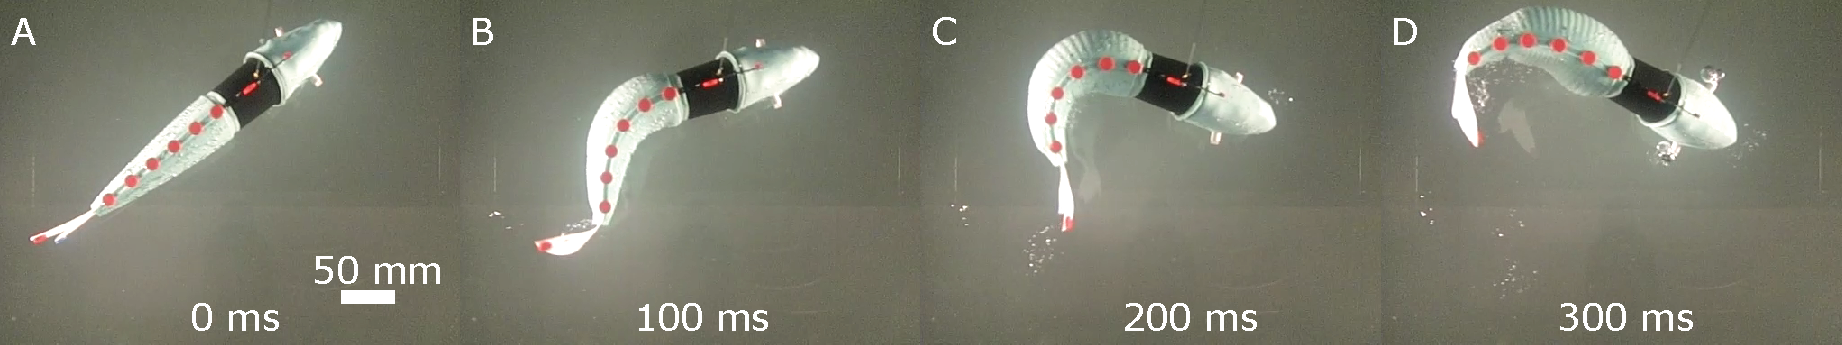
\includegraphics[width=0.9\columnwidth]{Figures/locomotion/pneumaticfish_escape_half.pdf}
            \caption{}
            \label{fig:pneumaticfish_escape}
        \end{subfigure}%
        \caption[Pneumatic Fish.]{A soft pneumatic robotic fish: (\textbf{a}) An overview of the robotic system, photo courtesy of Devon Jarvis, (\textbf{b}) A sequence depicting the fish performing an escape response.}
\end{figure}



\subsection{Hydraulic Fish}
\label{subsec:Locomotion, Hydraulic Fish}
The soft hydraulic fish~\cite{katzschmann2014hydraulic} with a single ribbed actuator is shown as a complete system in Figure~\ref{fig:hydraulic_fish_system_overview}. A close-up view is shown in Figure~\ref{fig:hydraulic_fish_yaw} and the 3d swimming capabilities are shown in Figure~\ref{fig:hydraulic_fish_all_motions}.

\begin{figure}[htb]
        \centering
        \begin{subfigure}[b]{0.48\columnwidth}
            \centering
           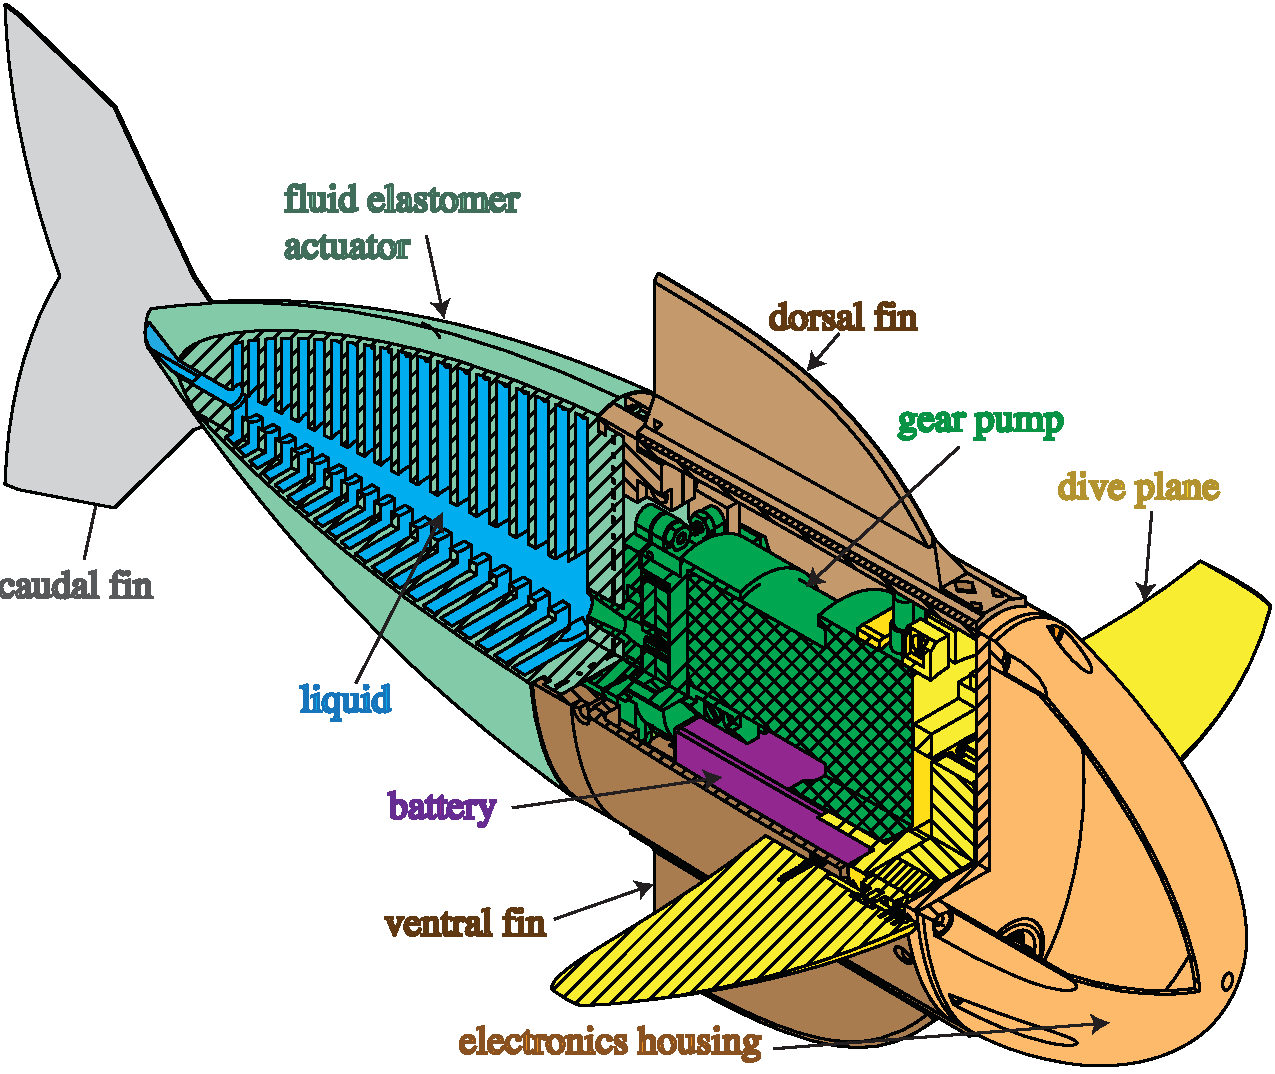
\includegraphics[width=1\columnwidth]{figures/locomotion/hydraulic_fish_system_overview.pdf}
           \caption{}
            \label{fig:hydraulic_fish_system_overview}
        \end{subfigure}
        \begin{subfigure}[b]{0.48\columnwidth}
            \centering
            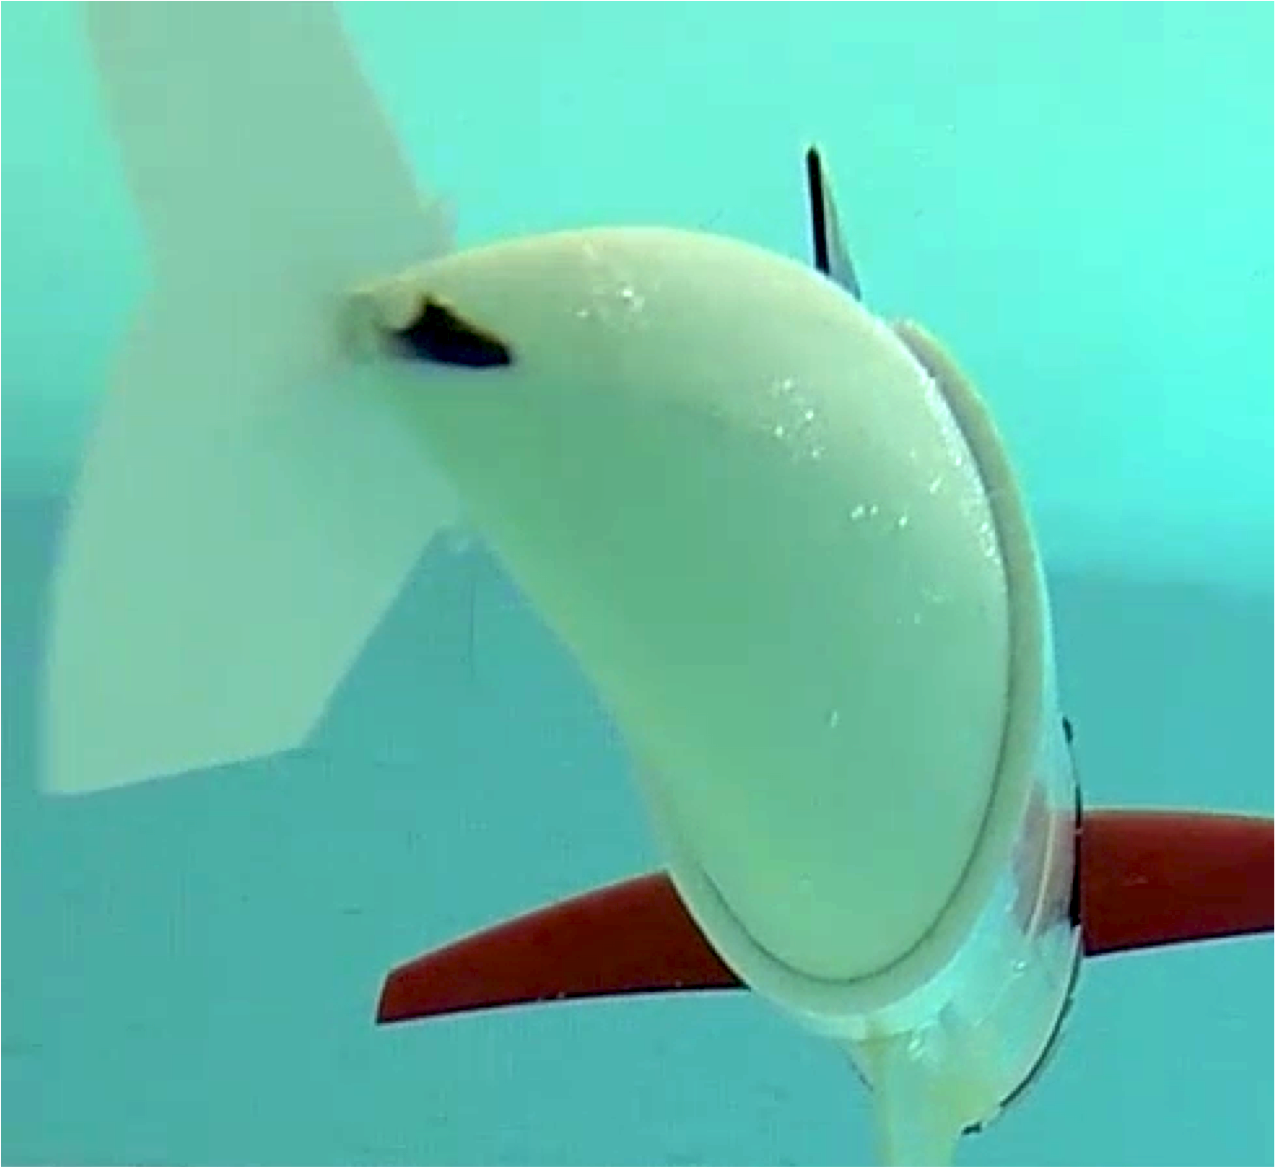
\includegraphics[width=1\columnwidth]{figures/locomotion/hydraulic_fish_yaw.png}
            \caption{}
            \label{fig:hydraulic_fish_yaw}
        \end{subfigure}\\
        \begin{subfigure}[b]{1\columnwidth}
            \centering
            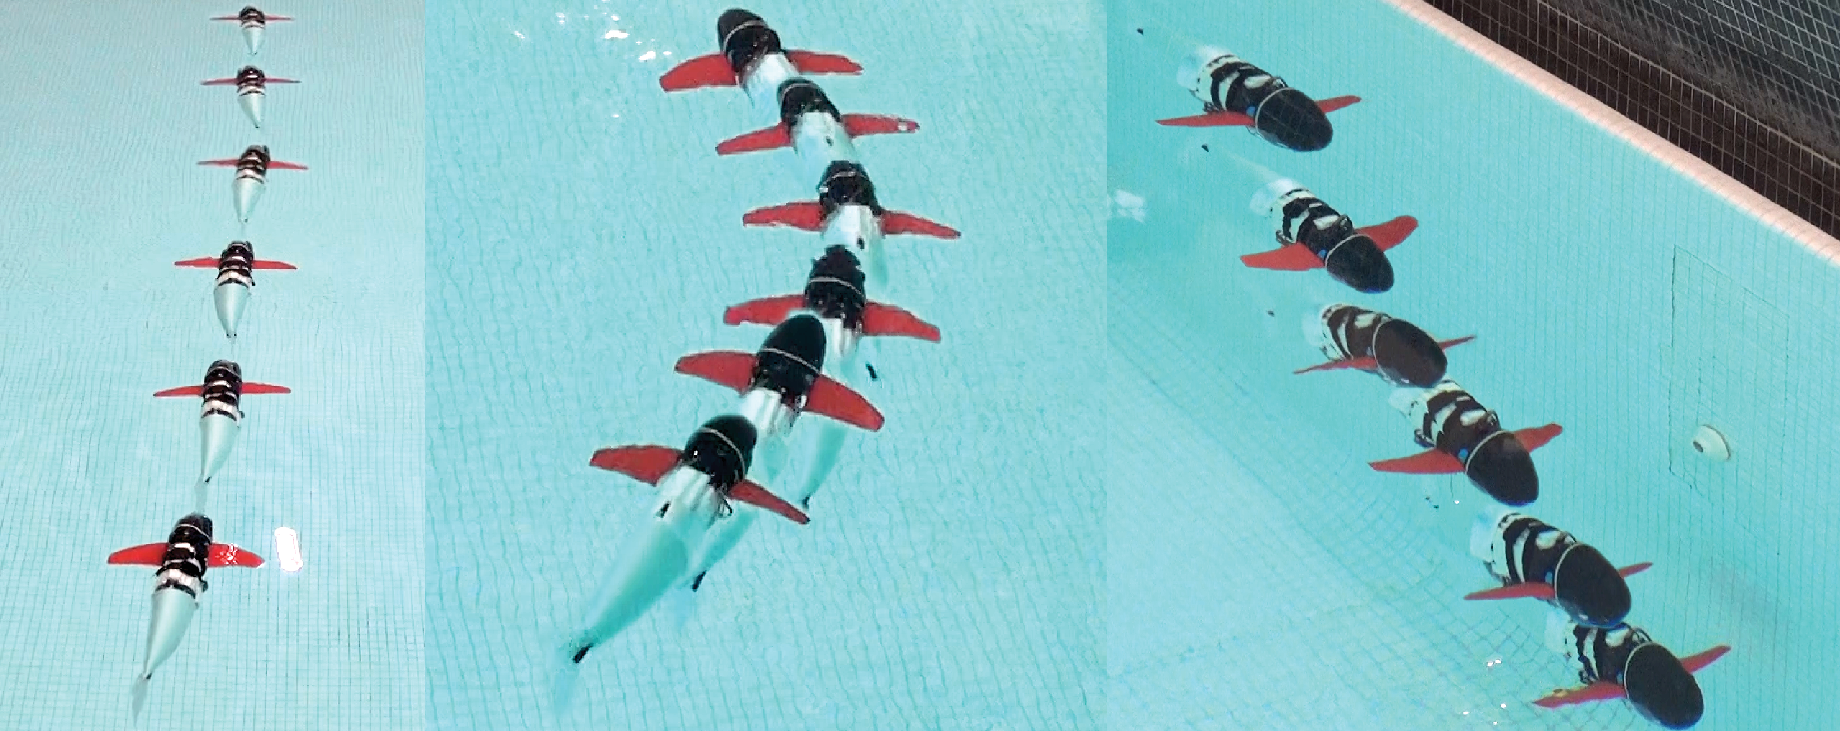
\includegraphics[width=1\columnwidth]{figures/locomotion/hydraulic_fish_all_motions.pdf}
            \caption{}
            \label{fig:hydraulic_fish_all_motions}
        \end{subfigure}%
        \caption[Hydraulic soft robotic fish]{A soft hydraulic robotic fish: (\textbf{a}) A schematic of the system, (\textbf{b}) underwater swimming motion, and (\textbf{c}) example of continuous forward swimming, yaw motion, and diving.}
\end{figure} 

\section{Manipulators}
\label{sec:Manipulators}
Soft and continuously deformable manipulators can be assembled from bending fluidic elastomer segments.
Specifically, in this section we detail how multi-segment manipulators can be composed by serially concatenating the actuated segments that were presented in Section~\ref{subsec:Actuators, Actuator Morphologies}.

\subsection{Ribbed}
\label{subsec:Manipulators, Ribbed}
Structurally, a ribbed arm is composed of serially concatenated, homogeneous ribbed body segments.
In this work, the manipulator's reachable envelope is constrained to the x-y plane.
%, as shown in Section~\ref{sec:System Overview}.
By volume, over ninety-seven percent of the ribbed manipulator is soft silicone rubber, excluding the feet.
This manipulator is depicted in Figure~\ref{fig:ribbed_manipulator_design} and can theoretically be composed of any number of the aforementioned ribbed segments (Fig.~\ref{fig:ribbed_manipulator_design}e).
Practically, we have constructed a six-segment prototype (Fig. \ref{fig:ribbed_manipulator_real}).
All twelve fluidic transmission lines as well as channel-to-supply interfaces are embedded within the manipulator's center layer.
Markers are located at the interface between segments (Fig.~\ref{fig:ribbed_manipulator_design}b), making segment endpoints identifiable to an external localization system.
The starting point of the arm's first segment (Fig.~\ref{fig:ribbed_manipulator_design}a) is grounded to the platform on which the arm moves and we refer to this as the base.
Ball transfers (Fig.~\ref{fig:ribbed_manipulator_design}d) are also located at each segment endpoint to allow the arm to move on a two-dimensional plane with minimal friction.
In many experiments conducted throughout this work, the pose of the arm's end-effector (Fig.~\ref{fig:ribbed_manipulator_design}c) is controlled.

\begin{figure}[htb]
        \centering
        \begin{subfigure}[b]{\columnwidth}
            \centering
            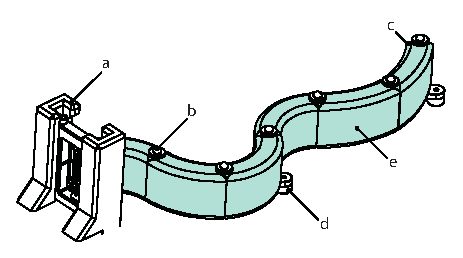
\includegraphics[width=0.9\columnwidth]{figures/manipulators/ribbed_manipulator}
            \caption{}
            \label{fig:ribbed_manipulator_design}
        \end{subfigure}\\
        \begin{subfigure}[b]{\columnwidth}
            \centering
            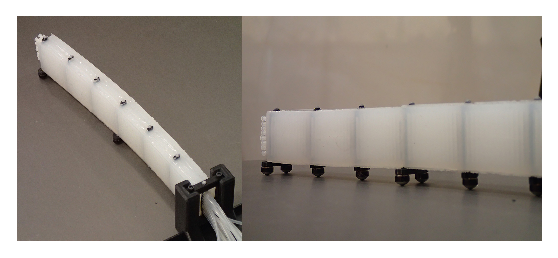
\includegraphics[width=0.9\columnwidth]{figures/manipulators/ribbed_manipulator_real}
            \caption{}
            \label{fig:ribbed_manipulator_real}
        \end{subfigure}%
        \caption[A ribbed soft manipulator prototype.]{A ribbed soft manipulator prototype. (\textbf{a}) The arm is composed of homogeneous and independently actuated ribbed segments (e). The base of the arm's first segment is fixed (a) and the end of its last segment is the end-effector (c). Markers (b) identify the endpoints of each segment and ball transfers (d) mitigate friction. (\textbf{b}) Photographs of the ribbed manipulator prototype.}
\end{figure}

\subsection{Cylindrical}
\label{subsec:Manipulators, Cylindrical}
We can also compose a manipulator from cylindrical fluidic elastomer segments, as shown in Figure~\ref{fig:cylindrical_manipulator}.
Just as in the ribbed composition, cylindrical segments are joined end-to-end.
Here, fluid transmission lines are passed through the manipulator's hollow center.
This feature not only facilitates segment concatenation, but also allows for modular composition of a manipulator, because transmission lines are not permanently embedded within the elastomer.
Additionally, this manipulator type is only composed of soft silicone rubber as there is no inextensible constraint.
No other materials are used, except for the attached ball transfers to mitigate ground friction.
\begin{figure}[htb]
\centering
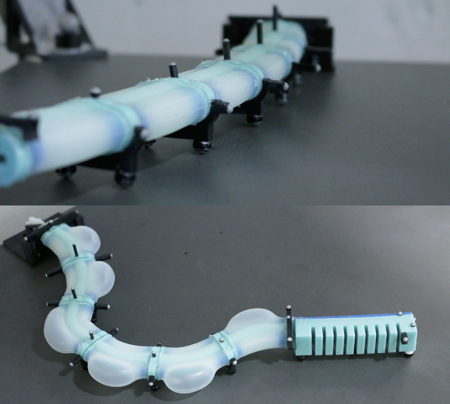
\includegraphics[width=\columnwidth]{Figures/manipulators/cylindrical_manipulator_real}
\caption[A cylindrical soft manipulator prototype.]{A cylindrical soft manipulator prototype with and without a pleated finger-like gripper.} \label{fig:cylindrical_manipulator}
\end{figure}

\subsection{Pleated}
\label{subsec:Manipulators, Pleated}
A manipulator can also be composed from pleated fluidic elastomer segments, as shown in Figure~\ref{fig:pleated_manipulator}.
Just as in the ribbed and cylindrical composition, pleated segments are joined end-to-end.
The fluid transmission lines are passed through along the central axis of the segments.
A supportive hollow profile can be added to combine two segments.
This pleated design allows for modular composition of a manipulator, because transmission lines are not permanently embedded within the elastomer.
Additionally, this type of manipulator is, like the cylindrical manipulator, composed entirely of soft silicone rubber.

\begin{figure}[htb]
\centering
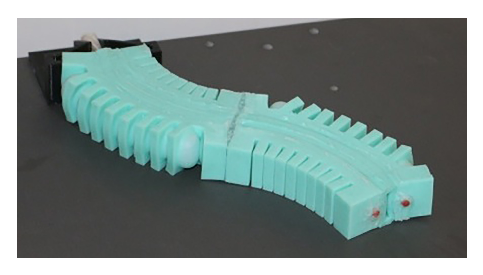
\includegraphics[width=\columnwidth]{Figures/manipulators/pleated_manipulator_real}
\caption[A pleated soft manipulator prototype.]{A pleated soft manipulator prototype, composed of two segments with two degrees of freedom each.}
\label{fig:pleated_manipulator}
\end{figure} 

%\input{capabilities}
%\clearpage

%\input{experimental_results}
%\clearpage

\section{Discussion}
\label{sec:discussion}
% What did we achieve?
The design of the actuators and fabrication methods described in this paper provide recipes for the rapid fabrication of modular soft robots with arbitrary body morphology.
%
%New capabilities
This class of soft robots is very well-suited for tasks requiring: (i) interactions with humans and environments to be safe, (ii) uncertainty to be mitigated at the hardware level, (iii) continuous and dexterous deformation, and/or (iv) hardware to take an unstructured, amorphous form.
%
For example, by making robots from soft elastic materials, with no sharp edges, and with relatively low link inertia, a robot's reliance on sensors and software for safety is reduced.
%
The prospects for safe integrations between a robot and human are generally increased when the compliance of the material composing the machine match those of soft biological materials \citet{majidi2014soft}, and this feature is inherent to robots made of soft silicone elastomer.
%
An alternative approach is to allow resilient soft machines to handle some uncertainty at the hardware level in order to reduce the burden on the computational system.
%
For example, consider how a soft manipulator passively conforms to the environment's boundary. The planner is unaware of this complex interaction, but the primary task can still be successfully executed.
%
Further, modern inspection tasks as well as invasive surgery require devices with redundant degrees of freedom and high dexterity and often impose the constraint of navigating around sensitive objects.
%
As initially demonstrated here, soft robotic manipulators may be well-suited for this class of tasks.

%What are the limitations and open problems



%Lastly, this work brings to attention the need for proprioceptive localization systems for soft robots. Feedback for our controller comes currently from an exteroceptive localization system. This is a reasonable method for indoor, laboratory or factory environments where there is sufficient line of sight to the manipulator. However, this sensor approach is prohibitive in that the environment must be equipped with cameras and the tasks cannot occlude the view of these cameras onto the manipulator. Proprioceptive localization for soft robots is an important avenue for future research.


\section*{Acknowledgments}
\label{sec:Acknowledgments}
This work was done in the Distributed Robotics Laboratory at MIT with support from the National Science Foundation, grant numbers NSF 1117178, NSF EAGER 1133224, NSF IIS1226883, and NSF CCF1138967 as well as NSF Graduate Research Fellowship Program, primary award number 1122374. We are grateful for this support. The authors declare no competing financial interests. 

%Photo in Figure~\ref{fig:intro_new}c courtesy of Devon Jarvis for Popular Mechanics. 

\bibliography{main}

\end{document}
